% Options for packages loaded elsewhere
\PassOptionsToPackage{unicode}{hyperref}
\PassOptionsToPackage{hyphens}{url}
%
\documentclass[
]{article}
\usepackage{lmodern}
\usepackage{amssymb,amsmath}
\usepackage{ifxetex,ifluatex}
\ifnum 0\ifxetex 1\fi\ifluatex 1\fi=0 % if pdftex
  \usepackage[T1]{fontenc}
  \usepackage[utf8]{inputenc}
  \usepackage{textcomp} % provide euro and other symbols
\else % if luatex or xetex
  \usepackage{unicode-math}
  \defaultfontfeatures{Scale=MatchLowercase}
  \defaultfontfeatures[\rmfamily]{Ligatures=TeX,Scale=1}
\fi
% Use upquote if available, for straight quotes in verbatim environments
\IfFileExists{upquote.sty}{\usepackage{upquote}}{}
\IfFileExists{microtype.sty}{% use microtype if available
  \usepackage[]{microtype}
  \UseMicrotypeSet[protrusion]{basicmath} % disable protrusion for tt fonts
}{}
\makeatletter
\@ifundefined{KOMAClassName}{% if non-KOMA class
  \IfFileExists{parskip.sty}{%
    \usepackage{parskip}
  }{% else
    \setlength{\parindent}{0pt}
    \setlength{\parskip}{6pt plus 2pt minus 1pt}}
}{% if KOMA class
  \KOMAoptions{parskip=half}}
\makeatother
\usepackage{xcolor}
\IfFileExists{xurl.sty}{\usepackage{xurl}}{} % add URL line breaks if available
\IfFileExists{bookmark.sty}{\usepackage{bookmark}}{\usepackage{hyperref}}
\hypersetup{
  pdftitle={Praktická časť diplomovej práce},
  hidelinks,
  pdfcreator={LaTeX via pandoc}}
\urlstyle{same} % disable monospaced font for URLs
\usepackage[margin=1in]{geometry}
\usepackage{color}
\usepackage{fancyvrb}
\newcommand{\VerbBar}{|}
\newcommand{\VERB}{\Verb[commandchars=\\\{\}]}
\DefineVerbatimEnvironment{Highlighting}{Verbatim}{commandchars=\\\{\}}
% Add ',fontsize=\small' for more characters per line
\usepackage{framed}
\definecolor{shadecolor}{RGB}{248,248,248}
\newenvironment{Shaded}{\begin{snugshade}}{\end{snugshade}}
\newcommand{\AlertTok}[1]{\textcolor[rgb]{0.94,0.16,0.16}{#1}}
\newcommand{\AnnotationTok}[1]{\textcolor[rgb]{0.56,0.35,0.01}{\textbf{\textit{#1}}}}
\newcommand{\AttributeTok}[1]{\textcolor[rgb]{0.77,0.63,0.00}{#1}}
\newcommand{\BaseNTok}[1]{\textcolor[rgb]{0.00,0.00,0.81}{#1}}
\newcommand{\BuiltInTok}[1]{#1}
\newcommand{\CharTok}[1]{\textcolor[rgb]{0.31,0.60,0.02}{#1}}
\newcommand{\CommentTok}[1]{\textcolor[rgb]{0.56,0.35,0.01}{\textit{#1}}}
\newcommand{\CommentVarTok}[1]{\textcolor[rgb]{0.56,0.35,0.01}{\textbf{\textit{#1}}}}
\newcommand{\ConstantTok}[1]{\textcolor[rgb]{0.00,0.00,0.00}{#1}}
\newcommand{\ControlFlowTok}[1]{\textcolor[rgb]{0.13,0.29,0.53}{\textbf{#1}}}
\newcommand{\DataTypeTok}[1]{\textcolor[rgb]{0.13,0.29,0.53}{#1}}
\newcommand{\DecValTok}[1]{\textcolor[rgb]{0.00,0.00,0.81}{#1}}
\newcommand{\DocumentationTok}[1]{\textcolor[rgb]{0.56,0.35,0.01}{\textbf{\textit{#1}}}}
\newcommand{\ErrorTok}[1]{\textcolor[rgb]{0.64,0.00,0.00}{\textbf{#1}}}
\newcommand{\ExtensionTok}[1]{#1}
\newcommand{\FloatTok}[1]{\textcolor[rgb]{0.00,0.00,0.81}{#1}}
\newcommand{\FunctionTok}[1]{\textcolor[rgb]{0.00,0.00,0.00}{#1}}
\newcommand{\ImportTok}[1]{#1}
\newcommand{\InformationTok}[1]{\textcolor[rgb]{0.56,0.35,0.01}{\textbf{\textit{#1}}}}
\newcommand{\KeywordTok}[1]{\textcolor[rgb]{0.13,0.29,0.53}{\textbf{#1}}}
\newcommand{\NormalTok}[1]{#1}
\newcommand{\OperatorTok}[1]{\textcolor[rgb]{0.81,0.36,0.00}{\textbf{#1}}}
\newcommand{\OtherTok}[1]{\textcolor[rgb]{0.56,0.35,0.01}{#1}}
\newcommand{\PreprocessorTok}[1]{\textcolor[rgb]{0.56,0.35,0.01}{\textit{#1}}}
\newcommand{\RegionMarkerTok}[1]{#1}
\newcommand{\SpecialCharTok}[1]{\textcolor[rgb]{0.00,0.00,0.00}{#1}}
\newcommand{\SpecialStringTok}[1]{\textcolor[rgb]{0.31,0.60,0.02}{#1}}
\newcommand{\StringTok}[1]{\textcolor[rgb]{0.31,0.60,0.02}{#1}}
\newcommand{\VariableTok}[1]{\textcolor[rgb]{0.00,0.00,0.00}{#1}}
\newcommand{\VerbatimStringTok}[1]{\textcolor[rgb]{0.31,0.60,0.02}{#1}}
\newcommand{\WarningTok}[1]{\textcolor[rgb]{0.56,0.35,0.01}{\textbf{\textit{#1}}}}
\usepackage{longtable,booktabs}
% Correct order of tables after \paragraph or \subparagraph
\usepackage{etoolbox}
\makeatletter
\patchcmd\longtable{\par}{\if@noskipsec\mbox{}\fi\par}{}{}
\makeatother
% Allow footnotes in longtable head/foot
\IfFileExists{footnotehyper.sty}{\usepackage{footnotehyper}}{\usepackage{footnote}}
\makesavenoteenv{longtable}
\usepackage{graphicx,grffile}
\makeatletter
\def\maxwidth{\ifdim\Gin@nat@width>\linewidth\linewidth\else\Gin@nat@width\fi}
\def\maxheight{\ifdim\Gin@nat@height>\textheight\textheight\else\Gin@nat@height\fi}
\makeatother
% Scale images if necessary, so that they will not overflow the page
% margins by default, and it is still possible to overwrite the defaults
% using explicit options in \includegraphics[width, height, ...]{}
\setkeys{Gin}{width=\maxwidth,height=\maxheight,keepaspectratio}
% Set default figure placement to htbp
\makeatletter
\def\fps@figure{htbp}
\makeatother
\setlength{\emergencystretch}{3em} % prevent overfull lines
\providecommand{\tightlist}{%
  \setlength{\itemsep}{0pt}\setlength{\parskip}{0pt}}
\setcounter{secnumdepth}{5}

\title{Praktická časť diplomovej práce}
\author{}
\date{\vspace{-2.5em}}

\begin{document}
\maketitle

\hypertarget{sprievodca-ekfmetriou}{%
\section{Sprievodca ekfmetriou}\label{sprievodca-ekfmetriou}}

Sprievodca ekonometriou má za úlohu priblížiť Vám ekonometriu, a pomôcť
Vám jej porozumieť. Sprievodcu píšem ako študent, ktorý sa ekonometriu
začal učiť sám, a sám si prešiel zdĺhavým procesom bádania a
usmerňovania. Sprievodca je zostrojený ako-tak súbežne s osnovou a
zadaniami, ktoré obdržíte na hodine. Nebudeme sa konkrétne držať
vypracovania zadaní, ale skôr princípmi, z ktorých zadania ťažia. Mnoho
študentov tento predmet nezaujíma, a zadania vypracujú okopírovaním
postupov starších spolužiakov, nuž, pochopiť ekonometriu a jej postupy
nie je vôbec jednoduché, a dokážem pochopiť, keď si študenti hľadajú
skratky. Na druhú stranu, ekonometria predstavuje skvelú vstupnú bránu
do sveta analytiky. Človek je zavalený Machine Learningom, Data Sciencom
a AI-čkom, nuž až po sfúknutí pozlátka zistí, že je to zmes matematiky,
štatistiky a počítačovej vedy (CS -- computer science). Ekonometria je
teda skvelou výhovorkou, ako oprášiť matematiku, doučiť sa štatistiku, a
naučiť sa troška programovania. R-ko sa môže zdať ako jazyk, ktorý žije
v tieni Pythonu, avšak, akoby nejedna Dominika vedela povedať, netreba
sa nechať voviesť do omylu. R-ko je najvhodnejší programovací jazyk pre
štatistikov, Google ho zahrnul do najnovších kurzov Google Analytics.
Mojou úlohou je pomôcť Vám prekonať problém, ktorý som na začiatku
svojej cesty ekonometriou vôbec nepovažoval za problém, a to množstvo
materiálov, ktoré zavalí študenta. Pomôžem Vám postupne zložiť skladačku
konceptov a teórií, na ktorých ekonometria stojí. Náročnosť
prezentovania konceptov bude prispôsobená. Nemá zmysel vysvetľovať
odvodzovanie každého estimátora. Cieľom je poskytnúť všeobecný náhľad
ekonometrie, a pomôcť Vám pochopiť, a teda príjemnejšie zvládnuť predmet
Ekonometria.

~

\textbf{Čo nás čaká:}

\begin{itemize}
\tightlist
\item
  Základy programovania v R\\
\item
  Intuitívny prehľad štatistických konceptov\\
\item
  Ekonometrické techniky
\end{itemize}

\newpage

\hypertarget{zuxe1klady-programovania-v-r}{%
\section{Základy programovania v R}\label{zuxe1klady-programovania-v-r}}

\begin{quote}
Sprievodca je interaktívny, teda začneme stiahnutím a inštaláciou
\href{https://cran.r-project.org/mirrors.html}{R} a
\href{https://cran.r-project.org/mirrors.html}{RStudia}. R má samo o
sebe programovacie prostredie, avšak dnešným štandardom je používanie
intregrovaného vývojového prostredia (IDE) v podobe RStudia.
\end{quote}

\hypertarget{aritmetickuxe9-operuxe1tory}{%
\subsection{Aritmetické operátory}\label{aritmetickuxe9-operuxe1tory}}

\emph{Poďme teda rovno na vec. Začneme základnými funkciami.} R môžeme
používať ako kalkulačku, teda za pomoci klasických aritmetických
operátorov môžeme sčítať, odčítať, násobiť, deliť či umocňovať:

\begin{Shaded}
\begin{Highlighting}[]
\DecValTok{5} \OperatorTok{+}\StringTok{ }\DecValTok{5}
\end{Highlighting}
\end{Shaded}

\begin{verbatim}
## [1] 10
\end{verbatim}

\begin{Shaded}
\begin{Highlighting}[]
\DecValTok{5} \OperatorTok{-}\StringTok{ }\DecValTok{5}
\end{Highlighting}
\end{Shaded}

\begin{verbatim}
## [1] 0
\end{verbatim}

\begin{Shaded}
\begin{Highlighting}[]
\DecValTok{5} \OperatorTok{*}\StringTok{ }\DecValTok{5}
\end{Highlighting}
\end{Shaded}

\begin{verbatim}
## [1] 25
\end{verbatim}

\begin{Shaded}
\begin{Highlighting}[]
\DecValTok{5} \OperatorTok{/}\StringTok{ }\DecValTok{5}
\end{Highlighting}
\end{Shaded}

\begin{verbatim}
## [1] 1
\end{verbatim}

\begin{Shaded}
\begin{Highlighting}[]
\DecValTok{5}\OperatorTok{^}\DecValTok{2}
\end{Highlighting}
\end{Shaded}

\begin{verbatim}
## [1] 25
\end{verbatim}

R-ko dokáže používať aj ďalšie aritmetické operátory:

\begin{Shaded}
\begin{Highlighting}[]
\CommentTok{# zobrazí zvyšok z delenia}

\DecValTok{5} \OperatorTok\StringTok{ }\DecValTok{2}
\end{Highlighting}
\end{Shaded}

\begin{verbatim}
## [1] 1
\end{verbatim}

My sa budeme zapodievať len tým, s čím sa na cvičeniach stretneme. Našou
úlohou nie je naučiť sa dokonalo ovládať R, ale naučiť sa používať ho v
dostatočnej miere, aby sme s ním zvládli to, čo budeme v najbližšej dobe
potrebovať.

\newpage

\hypertarget{baluxedky}{%
\subsection{Balíky}\label{baluxedky}}

Okrem základných operátorov budeme využívať aj funkcie:

\begin{Shaded}
\begin{Highlighting}[]
\KeywordTok{mean}\NormalTok{(}\DecValTok{2}\NormalTok{, }\DecValTok{4}\NormalTok{, }\DecValTok{6}\NormalTok{)}
\end{Highlighting}
\end{Shaded}

\begin{verbatim}
## [1] 2
\end{verbatim}

\begin{Shaded}
\begin{Highlighting}[]
\KeywordTok{abs}\NormalTok{(}\OperatorTok{-}\DecValTok{5}\NormalTok{)}
\end{Highlighting}
\end{Shaded}

\begin{verbatim}
## [1] 5
\end{verbatim}

\begin{Shaded}
\begin{Highlighting}[]
\KeywordTok{sqrt}\NormalTok{(}\DecValTok{8}\NormalTok{)}
\end{Highlighting}
\end{Shaded}

\begin{verbatim}
## [1] 2.828427
\end{verbatim}

Tieto funkcie sa nachádzajú v balíkoch, ktoré si môžeme predstaviť ako
také Addony. R figuruje balíkmi, ktoré sú predinštalované, a zahŕňajú
najpoužívanejšie a najzákladnejšie funkcie. Vyššie použíté funkcie sa
nachádzajú v balíku base. To, v akom balíku sa funkcia nachádza zistíte
po napísaní funkcie

~

\begin{center}


\includegraphics{diplomka obrazky/1.png}

\end{center}

~

to však len zapredpokladu, že už máte balík nainštalovaný. Ak narazíte
na názov funkcie, ktorú chcete použiť, avšak nemáte nainštalovaný balík
a chcete zistiť jeho názov, buď si funkciu zadajte do Google, alebo
napíšte do konzoly:

\begin{Shaded}
\begin{Highlighting}[]
\CommentTok{# ??meno funkcie}

\NormalTok{??mean}
\end{Highlighting}
\end{Shaded}

My budeme často využívať predinštalované balíky \textbf{base} a
\textbf{stats}, avšak za pochodu si budeme inštalovať aj ďalšie balíky,
s ktorými sa na cvičeniach stretnete. Nový balík je potrebné prv
nainštalovať a potom ho načítať do prostredia.

\begin{Shaded}
\begin{Highlighting}[]
\CommentTok{# stiahneme a našintalujeme pomocou R konzoly a funkcie install.packages()}
\CommentTok{# ! názov balíka je citlivý na veľkosť písma}
\CommentTok{# ! názov musí byť v úvodzovkách}

\KeywordTok{install.packages}\NormalTok{(}\StringTok{"fBasics"}\NormalTok{)}

\CommentTok{# po nainštalovaní máme balík stiahnutý v našom PC, a tento príkaz už viac nepoužívame}
\CommentTok{# ak však chceme funkcie z balíka použiť, musíme po zapnutí R-ka balík načítať príkazom}

\KeywordTok{library}\NormalTok{(fBasics)}

\CommentTok{# ! tu už úvodzovky nie sú potrebné}
\end{Highlighting}
\end{Shaded}

\begin{quote}
\emph{Pri inštalovaní názov balíka zabalíme do úvodzoviek. Pri jeho
načítaní pomocou library() už úvodzovky nepíšeme. Na pohovor si vezmeme
oblek (úvodzovky), ale po prijatí už chodíme do práce bez obleku.}
\end{quote}

\hypertarget{objekty}{%
\subsection{Objekty}\label{objekty}}

Často chceme vyrátané výsledky znova použiť, a preto by bolo vhodné si
ich niekde uložiť. Na ukladanie a uskladnenie výsledkov slúžia objekty.
Každý objekt má meno a obsah. Meno si môžeme zadať akékoľvek, musí však:

\begin{itemize}
\tightlist
\item
  začínať malým alebo veľkým písmenom a nie číslom
\item
  obsahovať iba čísla, písmená alebo niektoré špeciálne znaky ako
  \("."\) či "\_".
\end{itemize}

\begin{quote}
\emph{Nezabúdajme, že R je case sensitive (rozlišuje veľké a malé
písmená).}
\end{quote}

Povedzme že chceme vytvoriť objekt \textbf{a} a priradiť mu hodnotu
\(2 + 2\). Na priradenie obsahu je možné použiť \("="\), avšak
štandardom je používanie \("<-"\).

\begin{quote}
\emph{Znak \textless- nie je nutné písať dvoma znakmi, používa sa na to
skratka \textbf{``ľavý Alt'' a ``-''}. Na SK klávesnici nájdeme znak
naľavo od pravého Shiftu, na EN klávesnici zvyčajne naľavo od Backspacu.
Osobne programujem s EN klávesnicou, nech som použíteľný v akomkoľvek
štáte bez potreby inštalovať SK klávesnicu.}
\end{quote}

\begin{Shaded}
\begin{Highlighting}[]
\CommentTok{# Priradíme teda objektu "a" výsledok "2 + 2".}

\NormalTok{a <-}\StringTok{ }\DecValTok{2} \OperatorTok{+}\StringTok{ }\DecValTok{2}

\CommentTok{# Po napísaní názvu objektu do konzoly nám konzola ukáže už len výsledok.}

\NormalTok{a}
\end{Highlighting}
\end{Shaded}

\begin{verbatim}
## [1] 4
\end{verbatim}

\begin{Shaded}
\begin{Highlighting}[]
\CommentTok{# Nové priradenie hodnoty starému objektu prepíše starú hodnotu.}

\NormalTok{a <-}\StringTok{ }\DecValTok{5} \OperatorTok{+}\StringTok{ }\DecValTok{5}

\NormalTok{a}
\end{Highlighting}
\end{Shaded}

\begin{verbatim}
## [1] 10
\end{verbatim}

S daným objektom môžeme pracovať, akoby to bola číselná hodnota.

\begin{Shaded}
\begin{Highlighting}[]
\NormalTok{a}\OperatorTok{^}\DecValTok{2}
\end{Highlighting}
\end{Shaded}

\begin{verbatim}
## [1] 100
\end{verbatim}

\newpage

\hypertarget{vektory}{%
\subsection{Vektory}\label{vektory}}

Pre priradenie viacerých hodnôt vytvoríme vektor. Vektor vytvoríme
pomocou funkcie c() ako combine.

\begin{Shaded}
\begin{Highlighting}[]
\CommentTok{# Objektu "a" priradíme súbor číselných hodnôt a vytvoríme z neho vektor.}

\NormalTok{a <-}\StringTok{ }\KeywordTok{c}\NormalTok{(}\DecValTok{5}\NormalTok{, }\DecValTok{1}\NormalTok{, }\DecValTok{4}\NormalTok{, }\DecValTok{2}\NormalTok{, }\DecValTok{3}\NormalTok{)}

\NormalTok{a}
\end{Highlighting}
\end{Shaded}

\begin{verbatim}
## [1] 5 1 4 2 3
\end{verbatim}

S vektormi dokážeme rôzne pracovať. Sčítavať, násobiť, aplikovať na ne
funkcie, všetko, čo nás napadne. Ups, čo nám napadne!

\begin{Shaded}
\begin{Highlighting}[]
\NormalTok{b <-}\StringTok{ }\KeywordTok{c}\NormalTok{(}\DecValTok{5}\NormalTok{, }\DecValTok{9}\NormalTok{, }\DecValTok{6}\NormalTok{, }\DecValTok{8}\NormalTok{, }\DecValTok{7}\NormalTok{)}
\NormalTok{a }\OperatorTok{+}\StringTok{ }\NormalTok{b}
\end{Highlighting}
\end{Shaded}

\begin{verbatim}
## [1] 10 10 10 10 10
\end{verbatim}

\begin{Shaded}
\begin{Highlighting}[]
\KeywordTok{min}\NormalTok{(a)}
\end{Highlighting}
\end{Shaded}

\begin{verbatim}
## [1] 1
\end{verbatim}

\begin{Shaded}
\begin{Highlighting}[]
\KeywordTok{sort}\NormalTok{(a)}
\end{Highlighting}
\end{Shaded}

\begin{verbatim}
## [1] 1 2 3 4 5
\end{verbatim}

\begin{Shaded}
\begin{Highlighting}[]
\KeywordTok{sum}\NormalTok{(a)}
\end{Highlighting}
\end{Shaded}

\begin{verbatim}
## [1] 15
\end{verbatim}

Je vhodné poznať pár špeciálnych funkcií na tvorbu vektorov. A to:

\begin{Shaded}
\begin{Highlighting}[]
\CommentTok{# sample(), seq() a rep()}
\end{Highlighting}
\end{Shaded}

Často si totižto potrebujete vytvoriť vektor hodnôt podľa vlastnej
potreby. Hm, to som veľmi nič nové nepovedal. Ale\ldots{} Čo vlastne
tieto funkcie robia? A ako to zistíme? Ak pracujete s úplne novou
funkciou, a máte už nainštalovaný balík, a taktiež ste ho už načítali do
knižnice cez \(library()\), je vhodné použiť \(?názovfunkcie\) alebo
\(help(názovfunkcie)\). Poskytne Vám to stručný popis, čo funkcia robí,
všetky jej argumeny a aj pár príkladov. Ak už ste však s funkciou
pracovali, ale nepamätáte si argumenty, rozpíšte funkciu, kliknite sa do
zátvoriek funkcie \(mean(tu.sa.kliknete)\), a stlačíte \(TAB\). Vyhodí
Vám to argumenty funkcie. Skúsime si to na funkcii \(sample()\).

~

\hypertarget{sample}{%
\subsubsection{sample()}\label{sample}}

\begin{center}

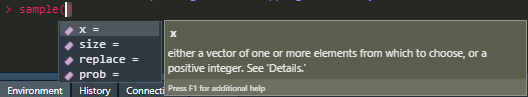
\includegraphics[width=0.85\textwidth,height=\textheight]{diplomka obrazky/2.png}

\end{center}

~

Pri jednej z vecí, ktorú Vám chcem ukázať, budeme potrebovať vektor
výšky ľudí. Tak si ho teda vytvorme už teraz. Ešte predtým môžeme skúsiť
napísať do konzoly \(?sample\), čím zistíme, že funkcia \(sample()\) nám
náhodne vyberie hodnoty zo zadaného vektora.

~

\begin{center}

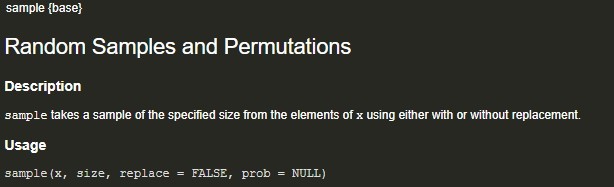
\includegraphics[width=0.8\textwidth,height=\textheight]{diplomka obrazky/3.png}

\end{center}

~

\begin{Shaded}
\begin{Highlighting}[]
\CommentTok{# Ako prvé potrebujeme zadať "x", teda vektor hodnôt, z ktorých chceme vyberať.}
\CommentTok{# Pre nás to budú hodnoty medzi 160 až 190, ktoré navolíme ako 160:190.}

\CommentTok{# 160:190 jednoducho vypíše hodnoty zaradom od 160 do 190. A sample() z nich náhodne vyberie}
\CommentTok{# nami určený počet hodnôt.}


\CommentTok{# "size" je počet hodnôt, aký ma funkcia vybrať.}

\CommentTok{# "replace", či môže vybrať jednu hodnotu viackrát, alebo ju má vylúčiť.}

\CommentTok{# "prob" použijeme, ak chceme priradiť istým hodnotám inú váhu.}

\NormalTok{vyska <-}\StringTok{ }\KeywordTok{sample}\NormalTok{(}\DataTypeTok{x =} \DecValTok{160}\OperatorTok{:}\DecValTok{190}\NormalTok{, }\DataTypeTok{size =} \DecValTok{10}\NormalTok{, }\DataTypeTok{replace =} \OtherTok{TRUE}\NormalTok{)}

\KeywordTok{print}\NormalTok{(vyska)}
\end{Highlighting}
\end{Shaded}

\begin{verbatim}
##  [1] 167 180 189 173 167 183 178 168 185 169
\end{verbatim}

\begin{quote}
\emph{Funkcia by fungovala, aj keby sme to napísali ako}
``sample(160:190, 10, TRUE)''. \emph{Je však vhodné písať aj argumenty.
Hlavne pri funkciách, ktoré nie sú veľmi bežné. Ak po Vás niekto bude
čítať kód, číta sa to lepšie.}
\end{quote}

\newpage

\hypertarget{seq}{%
\subsubsection{seq()}\label{seq}}

Funkcia \(seq()\) vygeneruje sekvenciu čísel. Ako argumenty zadávame buď
\(od\), \(do\) a \(by\). Teda po akých inkrementoch bude daná sekvencia
narastať.

\begin{Shaded}
\begin{Highlighting}[]
\KeywordTok{seq}\NormalTok{(}\DataTypeTok{from =} \DecValTok{2}\NormalTok{, }\DataTypeTok{to =} \DecValTok{12}\NormalTok{, }\DataTypeTok{by =} \FloatTok{0.5}\NormalTok{)}
\end{Highlighting}
\end{Shaded}

\begin{verbatim}
##  [1]  2.0  2.5  3.0  3.5  4.0  4.5  5.0  5.5  6.0  6.5  7.0  7.5  8.0  8.5  9.0
## [16]  9.5 10.0 10.5 11.0 11.5 12.0
\end{verbatim}

~

\begin{quote}
\emph{V Rku používame na oddeľovanie desatiných miest bodku. Čiarkou
oddeľujeme argumenty. Taktiež nezabúdajte používať medzery. Jedná sa o
gramatiku programovania. Predsalen náš vyššie napísaný výraz vyzerá
lepšie ako} seq(from=2,to=12,by=0.5).
\end{quote}

~

\begin{Shaded}
\begin{Highlighting}[]
\CommentTok{# Zadáme "od", "do" a koľko časí má vektor mať.}

\KeywordTok{seq}\NormalTok{(}\DataTypeTok{from =} \DecValTok{4}\NormalTok{, }\DataTypeTok{to =} \DecValTok{10}\NormalTok{, }\DataTypeTok{length =} \DecValTok{4}\NormalTok{) }
\end{Highlighting}
\end{Shaded}

\begin{verbatim}
## [1]  4  6  8 10
\end{verbatim}

\begin{Shaded}
\begin{Highlighting}[]
\KeywordTok{seq}\NormalTok{(}\DataTypeTok{from =} \DecValTok{4}\NormalTok{, }\DataTypeTok{to =} \DecValTok{10}\NormalTok{, }\DataTypeTok{length =} \DecValTok{8}\NormalTok{)}
\end{Highlighting}
\end{Shaded}

\begin{verbatim}
## [1]  4.000000  4.857143  5.714286  6.571429  7.428571  8.285714  9.142857
## [8] 10.000000
\end{verbatim}

\begin{Shaded}
\begin{Highlighting}[]
\CommentTok{# Alternatívou je zadať "od", "po", a rozdeliť to po požadovaných kúskoch}
\CommentTok{# na požadovanú dĺžku.}

\KeywordTok{seq}\NormalTok{(}\DataTypeTok{from =} \DecValTok{4}\NormalTok{, }\DataTypeTok{by =} \FloatTok{0.5}\NormalTok{, }\DataTypeTok{length =} \DecValTok{25}\NormalTok{)}
\end{Highlighting}
\end{Shaded}

\begin{verbatim}
##  [1]  4.0  4.5  5.0  5.5  6.0  6.5  7.0  7.5  8.0  8.5  9.0  9.5 10.0 10.5 11.0
## [16] 11.5 12.0 12.5 13.0 13.5 14.0 14.5 15.0 15.5 16.0
\end{verbatim}

\hypertarget{rep}{%
\subsubsection{rep()}\label{rep}}

Funkcie \(rep()\) jednoducho zopakuje zadané číslo, alebo vektor,
x-krát.

\begin{Shaded}
\begin{Highlighting}[]
\KeywordTok{rep}\NormalTok{(}\DataTypeTok{x =} \DecValTok{1}\NormalTok{, }\DataTypeTok{times =} \DecValTok{10}\NormalTok{)}
\end{Highlighting}
\end{Shaded}

\begin{verbatim}
##  [1] 1 1 1 1 1 1 1 1 1 1
\end{verbatim}

\begin{Shaded}
\begin{Highlighting}[]
\KeywordTok{rep}\NormalTok{(}\DataTypeTok{x =} \KeywordTok{c}\NormalTok{(}\DecValTok{1}\NormalTok{, }\DecValTok{2}\NormalTok{, }\DecValTok{3}\NormalTok{), }\DataTypeTok{times =} \DecValTok{3}\NormalTok{)}
\end{Highlighting}
\end{Shaded}

\begin{verbatim}
## [1] 1 2 3 1 2 3 1 2 3
\end{verbatim}

\hypertarget{indexovanie}{%
\subsection{Indexovanie}\label{indexovanie}}

Indexovanie je v R-ku veľmi užitočný spôsob selektovania dát. Ide
jednoducho o výber súboru dát, zo súboru dát. Indexujeme za použitia
hranatých zátvoriek, ktoré bez medzery nalepíme k objektu, z ktorého
chceme dáta vybrať. Najjednoduchšie sa to vysvetľuje ukážkou. A
nezabúdajte, že R-ko začína od jednotky, nie od nuly. Aj keď nám,
ekonómom neprogramátorom to asi ani nepríde divné.

\begin{Shaded}
\begin{Highlighting}[]
\CommentTok{# Vytvorme si obyčajný číselný vektor.}

\NormalTok{obycajny_vektor <-}\StringTok{ }\KeywordTok{c}\NormalTok{(}\DecValTok{1}\OperatorTok{:}\DecValTok{10}\NormalTok{)}

\NormalTok{obycajny_vektor}
\end{Highlighting}
\end{Shaded}

\begin{verbatim}
##  [1]  1  2  3  4  5  6  7  8  9 10
\end{verbatim}

\begin{Shaded}
\begin{Highlighting}[]
\CommentTok{# Za použitia indexovania môžeme vybrať akúkoľvek hodnotu. Chceme vybrať prvú.}

\NormalTok{obycajny_vektor[}\DecValTok{1}\NormalTok{]}
\end{Highlighting}
\end{Shaded}

\begin{verbatim}
## [1] 1
\end{verbatim}

\begin{Shaded}
\begin{Highlighting}[]
\CommentTok{# Alebo súbor hodnôt. Vyberieme prvú a poslednú hodnotu.}

\NormalTok{obycajny_vektor[}\KeywordTok{c}\NormalTok{(}\DecValTok{1}\NormalTok{, }\DecValTok{10}\NormalTok{)]}
\end{Highlighting}
\end{Shaded}

\begin{verbatim}
## [1]  1 10
\end{verbatim}

Pravdepodobne by väčšina z vás napísala \(obycajny\_vektor[1, 10]\), to
by vám však vyhodilo chybu. Prečo je tomu tak plne pochopíte, keď si
ukážeme matice. Aj keď to nie je nič zložité. Vektor si predstavme ako
šípku, ktorá určuje smer. Je to teda, v našom prípade, reťazec čísel,
jedna dlhá šnúra, ktorá nemá žiadne riadky ani stĺpce. R-ko však to, čo
napíšeme do hranatých zátvoriek vníma ako:

\[[riadok, stĺpec]\]\\
\[[row, column]\]

\begin{quote}
\emph{Zo začiatku sa mi zvyklo pliesť, čo ide prvé. Zapamätal som si to
ako RC autíčko. Také tie malé na ovládanie.}
\end{quote}

Čiže prvý údaj predstavuje riadok, a druhý údaj stĺpec. Ak by sme
napísali \([1, 10]\), R-ko by hľadalo v pŕvom riadku desiatu hodnotu. Do
hranatých zátvoriek píšeme vlastne \textbf{súradnice}. V reťazci hodnôt
máme ale iba reťazec hodnôt. (:D) Preto je potrebné použiť funkciu
\(c()\), aby R-ko vedelo, že má vyberať z reťazca hodnôt. Indexovanie je
veeeľmi užitočné, a dá sa využiť veľmi kreatívne. Nám však stačí vedieť,
čo to plus-mínus robí. Aby ste vedeli, čo sa deje, keď uvidíte hranaté
zátvorky. O indexovaní si ešte povieme pri maticiach.

\begin{Shaded}
\begin{Highlighting}[]
\CommentTok{# Indexovaním môžeme aj odobrať hodnotu. Napr., ak chceme všetky okrem poslednej:}

\NormalTok{obycajny_vektor[}\OperatorTok{-}\DecValTok{10}\NormalTok{]}
\end{Highlighting}
\end{Shaded}

\begin{verbatim}
## [1] 1 2 3 4 5 6 7 8 9
\end{verbatim}

\hypertarget{inuxe9-typy-vektorov}{%
\subsection{Iné typy vektorov}\label{inuxe9-typy-vektorov}}

Vektory nemusia obsahovať len čísla. Môžu obsahovať napríklad aj
\textbf{textové} alebo \textbf{logické} premenné. Existuje ešte aj
štvrtý typ, \textbf{faktorové} vektory, ktorým sa ale nebudeme zaoberať.

\hypertarget{vektor-textovuxfdch-premennuxfdch}{%
\subsubsection{Vektor textových
premenných}\label{vektor-textovuxfdch-premennuxfdch}}

\begin{Shaded}
\begin{Highlighting}[]
\CommentTok{# Pre vytvorenie vektora obsahujúceho textové reťazce, musí byť obsah ohraničený}
\CommentTok{# úvodzovkami "".}

\NormalTok{vector_characters <-}\StringTok{ }\KeywordTok{c}\NormalTok{(}\StringTok{"c"}\NormalTok{, }\StringTok{"musíme"}\NormalTok{, }\StringTok{"používať"}\NormalTok{, }\StringTok{"stále"}\NormalTok{, }\StringTok{"ak"}\NormalTok{, }\StringTok{"chceme"}\NormalTok{,}
                       \StringTok{"viac"}\NormalTok{, }\StringTok{"hodnôt"}\NormalTok{)}

\NormalTok{vector_characters}
\end{Highlighting}
\end{Shaded}

\begin{verbatim}
## [1] "c"        "musíme"   "používat" "stále"    "ak"       "chceme"   "viac"    
## [8] "hodnôt"
\end{verbatim}

Vektor tvorený textovým reťazcom nájde svoje uplatnenie napríklad pri
pomenovaní hodnôt.

\begin{Shaded}
\begin{Highlighting}[]
\NormalTok{nazvy <-}\StringTok{ }\KeywordTok{c}\NormalTok{(}\StringTok{"prvy"}\NormalTok{, }\StringTok{"druhy"}\NormalTok{, }\StringTok{"treti"}\NormalTok{)}
\NormalTok{cisla <-}\StringTok{ }\KeywordTok{c}\NormalTok{(}\DecValTok{1}\NormalTok{, }\DecValTok{2}\NormalTok{, }\DecValTok{3}\NormalTok{)}

\CommentTok{# Použijeme na to funkciu names()}

\KeywordTok{names}\NormalTok{(cisla) <-}\StringTok{ }\NormalTok{nazvy}

\CommentTok{# Ak sa teraz pozrieme na vektor "cisla", uvidíme, že sme číslam priradili názvy.}
\CommentTok{# Na vypísanie výsledku môžeme použíť aj funkciu print().}

\KeywordTok{print}\NormalTok{(cisla)}
\end{Highlighting}
\end{Shaded}

\begin{verbatim}
##  prvy druhy treti 
##     1     2     3
\end{verbatim}

Vektor \textbf{``cisla''} sme vlozili do funkcie \textbf{names()}.
Aplikovali sme funkciu na vektor, ktorému sme chceli priradiť názvy.
\textbf{Priradiť}, teda symbol priradenia \textbf{\textless-}, potom už
len vektor s názvami, ktoré chceme priradiť. Pre lepšiu ilustráciu si to
napíšeme nanovo, bez zadefinovaného vektora ``nazvy''.

\begin{Shaded}
\begin{Highlighting}[]
\KeywordTok{names}\NormalTok{(cisla) <-}\StringTok{ }\KeywordTok{c}\NormalTok{(}\StringTok{"adin"}\NormalTok{, }\StringTok{"dos"}\NormalTok{, }\StringTok{"tres"}\NormalTok{)}

\KeywordTok{print}\NormalTok{(cisla)}
\end{Highlighting}
\end{Shaded}

\begin{verbatim}
## adin  dos tres 
##    1    2    3
\end{verbatim}

\newpage

\hypertarget{vektor-logickuxfdch-premennuxfdch}{%
\subsubsection{Vektor logických
premenných}\label{vektor-logickuxfdch-premennuxfdch}}

\begin{Shaded}
\begin{Highlighting}[]
\CommentTok{# Logické operátory, inak známe ako Booleovské operátory, nám ako výsledok}
\CommentTok{# poskytnú výstup v podobe TRUE alebo FALSE.}
\CommentTok{# ! Pre overenie rovnosti použijeme "==".}

\NormalTok{vektor <-}\StringTok{  }\DecValTok{5}

\NormalTok{vektor }\OperatorTok{==}\StringTok{ }\DecValTok{5}
\end{Highlighting}
\end{Shaded}

\begin{verbatim}
## [1] TRUE
\end{verbatim}

\begin{Shaded}
\begin{Highlighting}[]
\NormalTok{vektor }\OperatorTok{==}\StringTok{ }\DecValTok{6}
\end{Highlighting}
\end{Shaded}

\begin{verbatim}
## [1] FALSE
\end{verbatim}

~

\begin{longtable}[]{@{}ll@{}}
\toprule
Logický operátor & Popis\tabularnewline
\midrule
\endhead
\textless{} & menšie než\tabularnewline
\textless= & menšie alebo rovné\tabularnewline
\textgreater{} & väčšie než\tabularnewline
\textgreater= & väčšie alebo rovné\tabularnewline
== & rovná sa\tabularnewline
!= & nerovná sa\tabularnewline
!x & nie je x\tabularnewline
x & y\tabularnewline
x \& y & x a y\tabularnewline
isTRUE(x) & test či je x pravdivé\tabularnewline
\bottomrule
\end{longtable}

~

Logické operátory sa zídu pri indexovaní, alebo pri zisťovaní počtu
vyhovujúcich hodnôt.

\begin{Shaded}
\begin{Highlighting}[]
\CommentTok{# Vektor výšky ľudí, ktorý sme si skôr vytvorili.}

\NormalTok{vyska <-}\StringTok{ }\KeywordTok{sample}\NormalTok{(}\DataTypeTok{x =} \DecValTok{160}\OperatorTok{:}\DecValTok{190}\NormalTok{, }\DataTypeTok{size =} \DecValTok{10}\NormalTok{, }\DataTypeTok{replace =} \OtherTok{TRUE}\NormalTok{)}

\CommentTok{# Použitie logického operátora na zistenie, kto má viac ako 170cm. }

\NormalTok{viac_ako_}\DecValTok{170}\NormalTok{ <-}\StringTok{ }\NormalTok{vyska }\OperatorTok{>}\StringTok{ }\DecValTok{170}

\CommentTok{# Výsledky však nebudú číselnými hodnotami, ale hodnotami booleovského typu.}

\KeywordTok{print}\NormalTok{(viac_ako_}\DecValTok{170}\NormalTok{)}
\end{Highlighting}
\end{Shaded}

\begin{verbatim}
##  [1]  TRUE  TRUE  TRUE  TRUE  TRUE  TRUE FALSE  TRUE  TRUE  TRUE
\end{verbatim}

\begin{Shaded}
\begin{Highlighting}[]
\CommentTok{# To nám však nebráni zužiťkovať to pomocou funkcie "sum()" a zistiť počet }
\CommentTok{# vyhovujúcich hodnôt. Zráta to všetky TRUE hodnoty.}

\KeywordTok{sum}\NormalTok{(viac_ako_}\DecValTok{170}\NormalTok{)}
\end{Highlighting}
\end{Shaded}

\begin{verbatim}
## [1] 9
\end{verbatim}

\begin{Shaded}
\begin{Highlighting}[]
\CommentTok{# Čo dokážeme pomocou indexovania pretvoriť na číselné hodnoty.}

\NormalTok{vyska_v_cm <-}\StringTok{ }\NormalTok{vyska[vyska }\OperatorTok{>}\StringTok{ }\DecValTok{170}\NormalTok{]}

\KeywordTok{print}\NormalTok{(vyska_v_cm)}
\end{Highlighting}
\end{Shaded}

\begin{verbatim}
## [1] 174 174 180 185 175 175 181 185 178
\end{verbatim}

\hypertarget{matice}{%
\subsection{Matice}\label{matice}}

\textbf{Matíc sa netreba ľakať.} Osobne som mal (vraj mal) v maticiach
isté medzery, a z mojich skúsenosti nie som jediný študent ekonómie s
týmto nedostatkom, nedostatkom vedomostí. Možno sa momentálne venujú
maticiam na predmete Matematika viac, nuž, aby som prešiel k veci, pre
zvládnutie základov ekonometrie nepotrebujete absolútne vedomosti matíc.
Ono, matica je len akási množina čísel usporiadaná do riadkov a stĺpcov
(rc, spomínate?), plus sa na ňu vzťahujú nejaké vlastnosti. Nejaké dosť
podstatné vlastnosti. Ako som ale vravel, netreba sa ľakať. My použijeme
matice, okrem iného, na počítanie Beta estimátorov v regresií by hand,
teda ručný výpočet nejakých hodnôt. Ak ste už zo štatistiky zabudli, čo
je regresia, tiež nevadí. Čo je regresia a prečo používame matice si
vysvetlíme neskôr. Teraz sa ich naučíme zostrojiť, a vysvetlíme si pár
\textbf{pojmov} a \textbf{vlastností} týkajúcich sa matíc, s ktorými sa
na hodinách stretnete.

\hypertarget{spuxf4soby-vytvuxe1rania-matice}{%
\subsubsection{Spôsoby vytvárania
matice}\label{spuxf4soby-vytvuxe1rania-matice}}

V aplikovanej ekonometrií sa matice väčšinou vytvárajú z existujúcich
datasetov. Vo všeobecnosti však máme tri možné spôsoby vytvárania matíc
v R. A to pomocou:

\begin{enumerate}
\def\labelenumi{\arabic{enumi}.}
\tightlist
\item
  funkcie \(matrix()\),
\item
  funkcie \(rbind()\),
\item
  funkcie \(cbind()\).
\end{enumerate}

\begin{Shaded}
\begin{Highlighting}[]
\CommentTok{# Pri funkcií matrix() zadáme vektor, a argumenty v podobe počtu riadkov, stĺpcov,}
\CommentTok{# a či má byť vektor usporiadaný po riadkoch alebo nie po riadkoch.}

\NormalTok{vektor <-}\StringTok{ }\KeywordTok{c}\NormalTok{(}\DecValTok{1}\NormalTok{, }\DecValTok{2}\NormalTok{, }\DecValTok{3}\NormalTok{, }\DecValTok{4}\NormalTok{, }\DecValTok{5}\NormalTok{, }\DecValTok{6}\NormalTok{, }\DecValTok{7}\NormalTok{, }\DecValTok{8}\NormalTok{, }\DecValTok{9}\NormalTok{)}

\CommentTok{# Vytvoríme si štvorcovú maticu 3x3}

\NormalTok{matica1 <-}\StringTok{ }\KeywordTok{matrix}\NormalTok{(vektor, }\DataTypeTok{nrow =} \DecValTok{3}\NormalTok{, }\DataTypeTok{ncol =} \DecValTok{3}\NormalTok{, }\DataTypeTok{byrow =} \OtherTok{TRUE}\NormalTok{)}

\NormalTok{matica1}
\end{Highlighting}
\end{Shaded}

\begin{verbatim}
##      [,1] [,2] [,3]
## [1,]    1    2    3
## [2,]    4    5    6
## [3,]    7    8    9
\end{verbatim}

\begin{Shaded}
\begin{Highlighting}[]
\CommentTok{# Zmeníme usporiadanie na FALSE, takže bude matica usporiadaná po stĺpcoch.}

\NormalTok{matica2 <-}\StringTok{ }\KeywordTok{matrix}\NormalTok{(vektor, }\DataTypeTok{nrow =} \DecValTok{3}\NormalTok{, }\DataTypeTok{ncol =} \DecValTok{3}\NormalTok{, }\DataTypeTok{byrow =} \OtherTok{FALSE}\NormalTok{)}

\NormalTok{matica2}
\end{Highlighting}
\end{Shaded}

\begin{verbatim}
##      [,1] [,2] [,3]
## [1,]    1    4    7
## [2,]    2    5    8
## [3,]    3    6    9
\end{verbatim}

Ďalšie dve funkcie fungujú na princípe zlepenia riadkov alebo stĺpcov
dohromady. Sú to intuitívne funkcie. Keďže bind znamená v preklade
spájať. Teda row bind, spájanie riadkov, a column bind ako spájanie
stĺpcov.

\begin{Shaded}
\begin{Highlighting}[]
\CommentTok{# Potrebujeme si vytvoriť vektory, ktoré budeme chcieť zlepiť.}
\CommentTok{# Vektor c(1:3) bude taký istý ako c(1, 2, 3).}

\NormalTok{vektor1 <-}\StringTok{ }\KeywordTok{c}\NormalTok{(}\DecValTok{1}\OperatorTok{:}\DecValTok{3}\NormalTok{)}
\NormalTok{vektor2 <-}\StringTok{ }\KeywordTok{c}\NormalTok{(}\DecValTok{4}\NormalTok{, }\DecValTok{5}\NormalTok{, }\DecValTok{6}\NormalTok{)}
\NormalTok{vektor3 <-}\StringTok{ }\KeywordTok{c}\NormalTok{(}\DecValTok{7}\NormalTok{, }\DecValTok{8}\NormalTok{, }\DecValTok{9}\NormalTok{)}

\CommentTok{# Zviazanie po riadkoch.}

\NormalTok{matica_riadky <-}\StringTok{ }\KeywordTok{rbind}\NormalTok{(vektor1, vektor2, vektor3)}

\NormalTok{matica_riadky}
\end{Highlighting}
\end{Shaded}

\begin{verbatim}
##         [,1] [,2] [,3]
## vektor1    1    2    3
## vektor2    4    5    6
## vektor3    7    8    9
\end{verbatim}

\begin{Shaded}
\begin{Highlighting}[]
\NormalTok{matica_stlpce <-}\StringTok{ }\KeywordTok{cbind}\NormalTok{(vektor1, vektor2, vektor3)}

\NormalTok{matica_stlpce}
\end{Highlighting}
\end{Shaded}

\begin{verbatim}
##      vektor1 vektor2 vektor3
## [1,]       1       4       7
## [2,]       2       5       8
## [3,]       3       6       9
\end{verbatim}

\hypertarget{indexovanie-1}{%
\subsubsection{Indexovanie}\label{indexovanie-1}}

Indexovanie matíc je veľmi intuitívne. Do hranatých zátvoriek zadáme ako
prvú hodnotu riadok, z ktorého chceme extrahovať hodnotu, a ako druhú
súradnicu zadáme stĺpec. Ak chceme vybrať celý riadok, zadáme len prvú
hodnotu, a druhú necháme prázdnu. Pri výbere celého stĺpca to funguje
presne naopak.

~

\begin{Shaded}
\begin{Highlighting}[]
\CommentTok{# Budeme pracovať s vyššie vytvorenou maticou "matica_riadky".}

\NormalTok{matica_riadky[}\DecValTok{1}\NormalTok{, }\DecValTok{3}\NormalTok{] }\CommentTok{# jeden prvok, prvý riadok, tretí stĺpec}
\end{Highlighting}
\end{Shaded}

\begin{verbatim}
## vektor1 
##       3
\end{verbatim}

\begin{Shaded}
\begin{Highlighting}[]
\NormalTok{matica_riadky[}\DecValTok{1}\NormalTok{, ] }\CommentTok{# celý prvý riadok}
\end{Highlighting}
\end{Shaded}

\begin{verbatim}
## [1] 1 2 3
\end{verbatim}

\begin{Shaded}
\begin{Highlighting}[]
\NormalTok{matica_riadky[ , }\DecValTok{1}\NormalTok{] }\CommentTok{# celý prvý stĺpec}
\end{Highlighting}
\end{Shaded}

\begin{verbatim}
## vektor1 vektor2 vektor3 
##       1       4       7
\end{verbatim}

\hypertarget{nuxe1sobenie-sux10duxedtanie-a-odux10duxedtanie-matuxedc}{%
\subsubsection{Násobenie, sčítanie a odčítanie
matíc}\label{nuxe1sobenie-sux10duxedtanie-a-odux10duxedtanie-matuxedc}}

Matice majú pĺno pravidiel. My si prejdeme len tie, na ktoré na
cvičeniach narazíme.

\begin{itemize}
\tightlist
\item
  Sčítavať a odčítavať môžeme iba matice, ktoré majú rovnaký počet
  riadkov a stĺpcov. Ako pri klasickom odčítaní neplatí, že:
  \(A - B = B - A\).
\item
  Pri násobení matíc musí platiť, že počet stĺpcov matice A musí byť
  zhodný s počtom riadkov matice B.

  \begin{itemize}
  \tightlist
  \item
    Výsledkom je potom matica, ktorá ma počet \textbf{r}iadkov ako prvá
    matica a počet stĺp\textbf{c}ov ako druhá matica, \textbf{rc} ;).
  \end{itemize}
\end{itemize}

\begin{center}

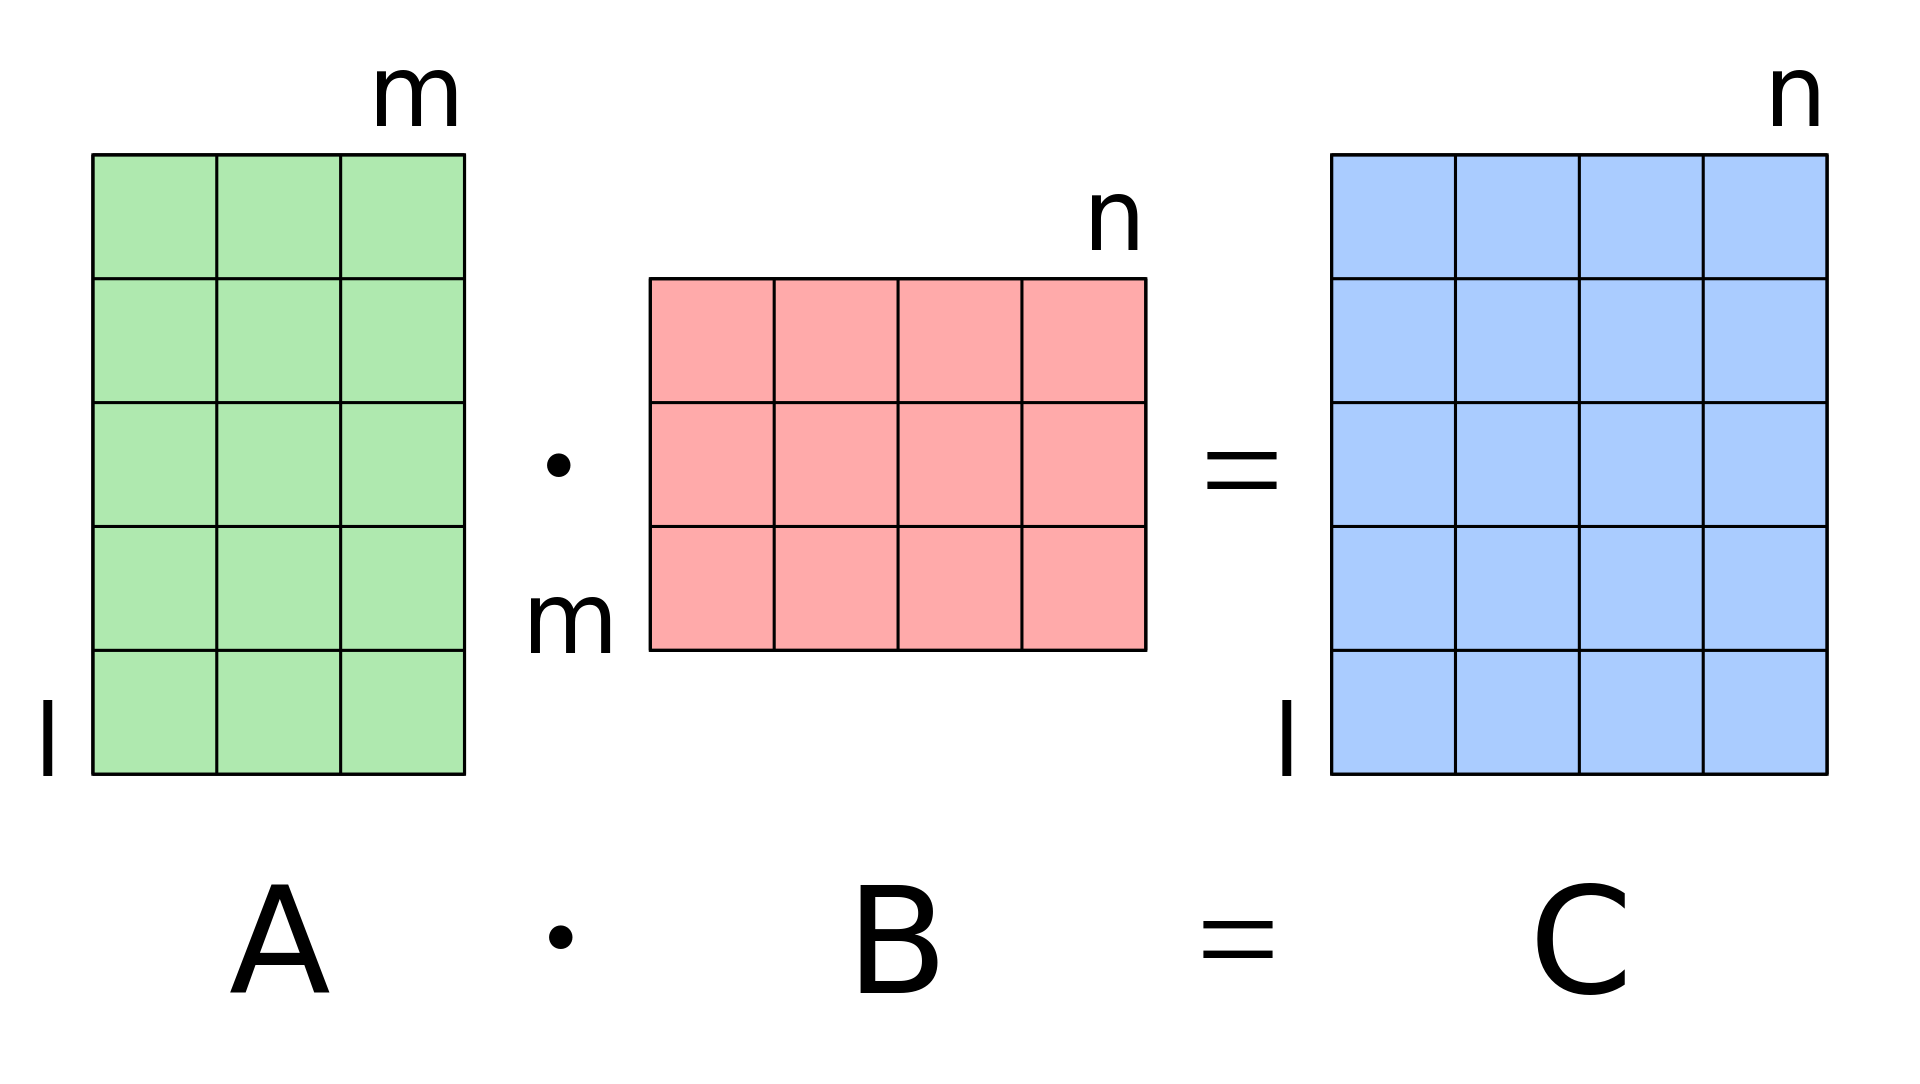
\includegraphics[width=0.5\textwidth,height=\textheight]{diplomka obrazky/4a.png}

\end{center}

Pri násobení matice skalárom, aka. jedným číslom, použijeme ako operátor
klasickú hviezdičku. Každý prvok matice bude prenásobený určeným číslom.

\begin{Shaded}
\begin{Highlighting}[]
\NormalTok{matica_riadky }\OperatorTok{*}\StringTok{ }\DecValTok{5}
\end{Highlighting}
\end{Shaded}

\begin{verbatim}
##         [,1] [,2] [,3]
## vektor1    5   10   15
## vektor2   20   25   30
## vektor3   35   40   45
\end{verbatim}

~

Pri násobení dvoch matíc sa používa trocha netradičný operátor
\(\%*\%\).

\begin{Shaded}
\begin{Highlighting}[]
\NormalTok{matica_riadky }\OperatorTok\StringTok{ }\NormalTok{matica_stlpce}
\end{Highlighting}
\end{Shaded}

\begin{verbatim}
##         vektor1 vektor2 vektor3
## vektor1      14      32      50
## vektor2      32      77     122
## vektor3      50     122     194
\end{verbatim}

~

Sčítanie matíc.

\begin{Shaded}
\begin{Highlighting}[]
\NormalTok{matica_riadky }\OperatorTok{+}\StringTok{ }\NormalTok{matica_stlpce}
\end{Highlighting}
\end{Shaded}

\begin{verbatim}
##         [,1] [,2] [,3]
## vektor1    2    6   10
## vektor2    6   10   14
## vektor3   10   14   18
\end{verbatim}

\hypertarget{transpozuxedcia-matice}{%
\subsubsection{Transpozícia matice}\label{transpozuxedcia-matice}}

Transponovaním matice dôjde k vzájomnej výmene riadkov a stĺpcov matice.
Takúto maticu označujeme ako \(A^T\). Ak bola prvotná matica (m, n), po
transpozícií vznikne matica s rozmermi (n, m). V R-ku matice
transponujeme pomocou funkcie t() ako transpose.

\begin{Shaded}
\begin{Highlighting}[]
\NormalTok{matica_riadky}
\end{Highlighting}
\end{Shaded}

\begin{verbatim}
##         [,1] [,2] [,3]
## vektor1    1    2    3
## vektor2    4    5    6
## vektor3    7    8    9
\end{verbatim}

\begin{Shaded}
\begin{Highlighting}[]
\KeywordTok{t}\NormalTok{(matica_riadky)}
\end{Highlighting}
\end{Shaded}

\begin{verbatim}
##      vektor1 vektor2 vektor3
## [1,]       1       4       7
## [2,]       2       5       8
## [3,]       3       6       9
\end{verbatim}

\hypertarget{hodnosux165-rank-matice}{%
\subsubsection{Hodnosť (rank) matice}\label{hodnosux165-rank-matice}}

V zadaniach od vás bude požadované vyrátať hodnosť matice, čo sa zvykne
označovať aj ako rank matice. Hodnosť matice je maximálny počet lineárne
nezávislých riadkov, alebo stĺpcov, v matici. Dva vektory
\(\overrightarrow{\text{a}}\), \(\overrightarrow{\text{b}}\) nazývame
lineárne závislé vektory práve vtedy, ak existuje reálne číslo \(k\)
také, že platí:

\[\overrightarrow{b} = k\overrightarrow{a}\]

Ak táto rovnosť neplatí, vektory sú lineárne nezávislé. Keď sme
spomínali maximálny počet buď riadkov alebo stĺpcov, mysleli sme tým, že
ak nepracujeme so štvorcovou maticou, maximálna hodnosť môže byť najviac
rovná tomu, čoho je menej. Ak máme maticu 3x4, jej maximálna hodnosť
môže byť 3. Lebo riadkov máme menej. Ak by sme mali maticu 4x2,
maximálna hodnosť môže byť 2. Hodnosť matice sa v R-ku vyráta pomocou
funkcie \(qr()\).

\begin{Shaded}
\begin{Highlighting}[]
\CommentTok{# Predpokladajme, že pracujeme so štvorcovou maticou.}
\CommentTok{# Ak by ste mali overiť, či sú vektory lineárne nezávislé,}
\CommentTok{# všetky ich spojíme do matice, a vyrátame rank matice. Ak bude rank}
\CommentTok{# rovný počtu vektorov, vektory sú navzájom  lineárne nezávislé.}

\NormalTok{vektor1 <-}\StringTok{ }\KeywordTok{c}\NormalTok{(}\DecValTok{2}\NormalTok{, }\DecValTok{3}\NormalTok{, }\DecValTok{1}\NormalTok{, }\DecValTok{9}\NormalTok{)}
\NormalTok{vektor2 <-}\StringTok{ }\KeywordTok{c}\NormalTok{(}\DecValTok{1}\NormalTok{, }\DecValTok{0}\NormalTok{, }\DecValTok{3}\NormalTok{, }\DecValTok{4}\NormalTok{)}
\NormalTok{vektor3 <-}\StringTok{ }\KeywordTok{c}\NormalTok{(}\DecValTok{2}\NormalTok{, }\DecValTok{9}\NormalTok{, }\DecValTok{0}\NormalTok{, }\DecValTok{3}\NormalTok{)}
\NormalTok{vektor4 <-}\StringTok{ }\KeywordTok{c}\NormalTok{(}\DecValTok{4}\NormalTok{, }\DecValTok{7}\NormalTok{, }\DecValTok{2}\NormalTok{, }\DecValTok{4}\NormalTok{)}

\NormalTok{matica <-}\StringTok{ }\KeywordTok{rbind}\NormalTok{(vektor1, vektor2, vektor3, vektor4)}


\CommentTok{# Operátor "$" dokáže extrahovať konkrétnu hodnotu, ktorú chceme extrahovať. Skúste použiť}
\CommentTok{# príkaz "qr(matica)", ktorý nám vyráta ešte pár ďalších vecí. Nás však zaujíma iba rank.}

\KeywordTok{qr}\NormalTok{(matica)}\OperatorTok{$}\NormalTok{rank }\CommentTok{# vyrátame hodnosť matice}
\end{Highlighting}
\end{Shaded}

\begin{verbatim}
## [1] 4
\end{verbatim}

\begin{Shaded}
\begin{Highlighting}[]
\CommentTok{# Vidíme, že rank je rovný počtu riadkov/stĺpcov, teda naše vektory sú lineárne nezávislé.}
\end{Highlighting}
\end{Shaded}

\hypertarget{determinant-matice}{%
\subsubsection{Determinant matice}\label{determinant-matice}}

Determinant matice si môžeme predstaviť ako hodnotu, ktorá je priradená
matici podľa toho, ako vyzerá. Matice môžu mať determinant nulový alebo
nenulový. Mohli by sme to rátať ručne, necháme to však R-ko vyrátať za
nás. Nás budú zaujímať aké vlastnosti sa s determinantom spájajú.

\hypertarget{inverznuxe1-matica}{%
\subsubsection{Inverzná matica}\label{inverznuxe1-matica}}

Inverzná matica je matica \(A^{-1}\), ktorá nám po vynásobení pôvodnou
maticou A, dá jednotkovú maticu. Funguje to aj naopak, teda platí vzťah:

\[A * A^{-1} = A^{-1} * A = E\]

Inverznú maticu vytvoríme pomocou funkcie \(solve()\)

\hypertarget{singuluxe1rna-reguluxe1rna-matica}{%
\subsubsection{Singulárna / Regulárna
matica}\label{singuluxe1rna-reguluxe1rna-matica}}

Ak je matica regulárna, znamená to, že má inverziu. Ak je singulárna,
nemá inverziu, teda \(A^{-1}\) neexistuje.

\begin{itemize}
\tightlist
\item
  Matica je singulárna ak:

  \begin{itemize}
  \tightlist
  \item
    má determinant rovný nule,
  \item
    sa hodnost nerovná poctu riadkov (ak má napr. 3x3 matica hodnost 2)
  \end{itemize}
\item
  Matica je regulárna ak:

  \begin{itemize}
  \tightlist
  \item
    má nenulový determinant,
  \item
    sa hodnost rovná poctu riadkov/stlpcov.
  \end{itemize}
\end{itemize}

\hypertarget{pruxe1ca-s-datasetmi-a-ich-analuxfdza}{%
\section{Práca s datasetmi a ich
analýza}\label{pruxe1ca-s-datasetmi-a-ich-analuxfdza}}

Vrhneme sa na:

\begin{itemize}
\tightlist
\item
  načítanie datasetov do R-ka a objektov,
\item
  manipuláciu datasetov,
\item
  vysvetlenie lineárneho regresného modelu,
\item
  prácu s regresnými modelmi.
\end{itemize}

\hypertarget{naux10duxedtanie-duxe1t}{%
\subsection{Načítanie dát}\label{naux10duxedtanie-duxe1t}}

Načítať dáta je možné rôznymi spôsobmi. V okne \(Environment\) môžete
kliknúť na \(Import \ dataset\) a vybrať typ súboru, aký chcete
importovať. Sofistikovanejšie je však načítavanie údajov pomocou
funkcií. Tých je tiež niekoľko, plus, existujú rôzne balíky, ktoré sú
vyvinuté na zlepšenie práce s dátami a ich vizáže. Vám však bude stačíť
jediná funkcia a to \(read.csv2\). Predtým než funkciu použijeme, si
však treba nastoliť isté štandardy. Ideálne je, aby ste mali vytvorenú
zložku, v ktorej budete mať všetky datasety (excelovské súbory) a pekne
oddelené zložky k cvičeniam. Nazývame to ``working directory'' AKA
pracovný adresár. Na zistenie, kde je Váš momentálny pracovný adresár
použijeme funkciu \(getwd()\) (get working directorty). Potrebujeme to
vedieť preto, lebo do funkcie \(read.csv2\) potrebujeme zadať argument
umiestnenia súboru. A je ľahšie zadať:

\begin{Shaded}
\begin{Highlighting}[]
\KeywordTok{read.csv2}\NormalTok{(}\StringTok{"udaje_o_pocte_kaciatok"}\NormalTok{)}

\CommentTok{# než}

\KeywordTok{read.csv2}\NormalTok{(}\StringTok{"C:/Desktop/MilanRozok/ekonometria/test/udaje_o_pocte_kaciatok.csv"}\NormalTok{)}
\end{Highlighting}
\end{Shaded}

Určenie nového adresára je možné urobiť pomocou \(setwd()\) (set working
directory), kde ako argument zadáme cestu do nového adresára, avšak,
jednoduchšie je kliknúť vľavo hore na:

\begin{center}

Session -\textgreater{} Set Working Directory -\textgreater{} Choose
directory,

\end{center}

a vybrať si adresár manuálne. Všetky datasety potom môžeme načítať
funkciou \(read.csv2()\) už len pomocou uvedenia názvu v úvodzovách, a
nemusíme uvádzať celú cestu umiestnenia súboru.

\hypertarget{read.csv2}{%
\subsubsection{read.csv2()}\label{read.csv2}}

Súbory typu .CSV znamenajú doslovne \(Comma-separated \ values\), teda
hodnoty oddelené čiarkami. Keď sa bavíme o formáte .CSV predstavte si
súbor, kde každá hodnota má svoj riadok, a každá premenná má svoj
stĺpec. Ako hodnoty sa chápe oddelenie stlpcov, teda stĺpce sú väčšinou
oddelené čiarkami. To je však taký teoretický prístup, v praxi môžu byť
tieto hodnoty oddelené aj inými spôsobmi. Hlavné však je pozerať na
koncovku súboru, resp. súbor (napr. z Excelu), uložiť ako .CSV súbor.
Funkcie \(read.csv()\) a \(read.csv2()\) robia to isté, jediné v čom sa
líšia je ich defaultné nastavenie. \(read.csv()\) ráta, že sa na
oddelenie desatinných miest používa bodka (čo je také americké), a
\(read.csv2()\), používa na oddelenie desatinných miest čiarku (čo je
také európske). To je dôvod, prečo primárne používame \(read.csv2()\).

\hypertarget{pruxe1ca-so-vstavanuxfdmi-datasetmi}{%
\subsubsection{Práca so vstavanými
datasetmi}\label{pruxe1ca-so-vstavanuxfdmi-datasetmi}}

R-ko obsahuje vstavané datasety, ktoré si môžeme všetky vypísať pomocou:

\begin{Shaded}
\begin{Highlighting}[]
\KeywordTok{data}\NormalTok{()}
\end{Highlighting}
\end{Shaded}

V tomto sprievodcovi budeme pracovať s dátami, ktoré si môžete načítať
zo vstavaného balíka \(datasets\). Je to z dôvodu, že je to proste
jednoduché. Na hodinách budete pracovať s pravými ekonomickými
datasetmi, avšak pre ukážku, ako čo funguje, a ako s čím súvisí nám
postačia základné datasety, ktoré sú ľahké na pochopenie. Ak si budete
chcieť overiť nejakú funkciu či teóriu, budete si môcť za pochodu
načítať dataset, s ktorým ste oboznámený, a otestovať, čo potrebujete.

\begin{Shaded}
\begin{Highlighting}[]
\CommentTok{# Pre načítanie datasetu do objektu použijeme trocha nezvyčajný prístup, kde:}
\CommentTok{# datasets predstavuje názov balíku, a "mtcars" dataset, ktorý chceme sprístupniť.}
\CommentTok{# Pomocou "::" sprístupníme konkrétny objekt z balíka.}

\NormalTok{data <-}\StringTok{ }\NormalTok{datasets}\OperatorTok{::}\NormalTok{mtcars}

\CommentTok{# Ak by sme datasetu nechceli priradiť vlastný názov, ale ponechať originálny:}

\KeywordTok{data}\NormalTok{(}\StringTok{"mtcars"}\NormalTok{)}

\CommentTok{# Funkcia bude fungovať aj bez úvodzoviek.}
\end{Highlighting}
\end{Shaded}

\hypertarget{jednoduchuxe1-lineuxe1rna-regresia}{%
\section{Jednoduchá lineárna
regresia}\label{jednoduchuxe1-lineuxe1rna-regresia}}

Hlavným nástrojom ekonometrie je regresia. Cieľom regresie je zistiť ako
určená/é nezávislé premenné, ovplyvňujú jednu závislú premennú. Ak \(Y\)
je závislá a \(X\) nezávislá, tak regresujeme, robíme regresiu, Y na X.
Čo však tá magická skrinka vlastne robí?

\begin{Shaded}
\begin{Highlighting}[]
\CommentTok{# Predpokladajme, že máme načítaný dataset "mtcars".}
\CommentTok{# Pomocou funkcie "head()" si načítame prvých 6 riadkov.}
\CommentTok{# Alternatíva je "tail()" (ako chvost), pre vypísanie posledných 6 riadkov.}

\KeywordTok{head}\NormalTok{(data)}
\end{Highlighting}
\end{Shaded}

\begin{verbatim}
##                    mpg cyl disp  hp drat    wt  qsec vs am gear carb
## Mazda RX4         21.0   6  160 110 3.90 2.620 16.46  0  1    4    4
## Mazda RX4 Wag     21.0   6  160 110 3.90 2.875 17.02  0  1    4    4
## Datsun 710        22.8   4  108  93 3.85 2.320 18.61  1  1    4    1
## Hornet 4 Drive    21.4   6  258 110 3.08 3.215 19.44  1  0    3    1
## Hornet Sportabout 18.7   8  360 175 3.15 3.440 17.02  0  0    3    2
## Valiant           18.1   6  225 105 2.76 3.460 20.22  1  0    3    1
\end{verbatim}

\begin{Shaded}
\begin{Highlighting}[]
\CommentTok{# Vidíme, že je to súbor aút, s rôznymi parametrami.}
\CommentTok{# My sa budeme snažiť vysvetliť vplyv "hp" (horsepower, konské sily), }
\CommentTok{# na "mph" (miles per galon, čiže koľko kilometrov má auto dojazd).}
\end{Highlighting}
\end{Shaded}

Pozrime sa na tento model:

\[y_i = \beta_0 + \beta{x_i} + \epsilon_i.\]

Jedná sa o základný model lineárnej regresie. Ak si bety predstavíme ako
obyčajné hodnoty, model v tomto jednoduchom znení by Vám z matematiky
mohol byť povedomý. Výsledkom modelu je priamka \(y\), kde \(\beta_0\)
je obyčajná hodnota v ktorej je os Y pretnutá, \(\beta_1\) určuje sklon
priamky. Keďže priamka nebude prechádzať každou nameranou hodnotou,
\(\epsilon\) v modeli znázorňuje tento priestor medzi meraniami a
priamkou. Označujeme ho ako náhodnú zložku. Môže byť spôsobená mnohými
spôsobmi. Okrem iného napríklad: chybným meraním, náhodou, alebo
premennými, ktoré sme do modelu nezahrnuli. Jedno auto so 150 koňskými
silami môže na plnú nádrž prejsť 500km a druhé len 350. Môže to byť
spôsobené váhou, avšak v modeli máme len výkon auta. Táto zložka sa v
priemere rovná nule, a z modelu nám odpadne (viac o tom neskôr). Tento
model si môžeme v našom príklade prepísať ako:

\[mpg_i = \beta_0 + \beta_1{hp_i} + \epsilon_i.\] Priamka, ktorá by
vznikla výsledkom tohto modelu sa nazýva populačná regresná priamka. Na
vyhodnotenie takéhoto modelu by sme však potrebovali dáta z celej
určenej populácie, čo je veľmi často prakticky nemožné. Vo všeobecnosti
sú populačné parametre \(\beta_0\) a \(\beta_1\) neznáme. Avšak dokážeme
ich odhadnúť pomocou estimátorov. Preto pracujeme so vzorkami, ktoré
dokážeme reálne odpozorovať a zozbierať. Estimátory zo vzorky dokážu
poskytnúť dostatočne dôveryhodné odhady koeficientu v populácií. Poďme
si to teda ukázať na našej vzorke.

Skúsme si hodiť do grafu výkon a dojazd, nech sa pozrieme na vzťah medzi
týmito premennými.

\begin{Shaded}
\begin{Highlighting}[]
\CommentTok{# Plotneme si dáta, ktoré dáme do regresie, čiže "mpg" a "hp".}

\KeywordTok{plot}\NormalTok{(}\DataTypeTok{x =}\NormalTok{ data}\OperatorTok{$}\NormalTok{hp, }\DataTypeTok{y =}\NormalTok{ data}\OperatorTok{$}\NormalTok{mpg, }\DataTypeTok{ylab =} \StringTok{"ylab ako y label"}\NormalTok{, }\DataTypeTok{xlab =} \StringTok{"tu máme výkon",}
\StringTok{     main = "}\NormalTok{Vzťah dojazdu a výkonu motora}\StringTok{")}
\end{Highlighting}
\end{Shaded}

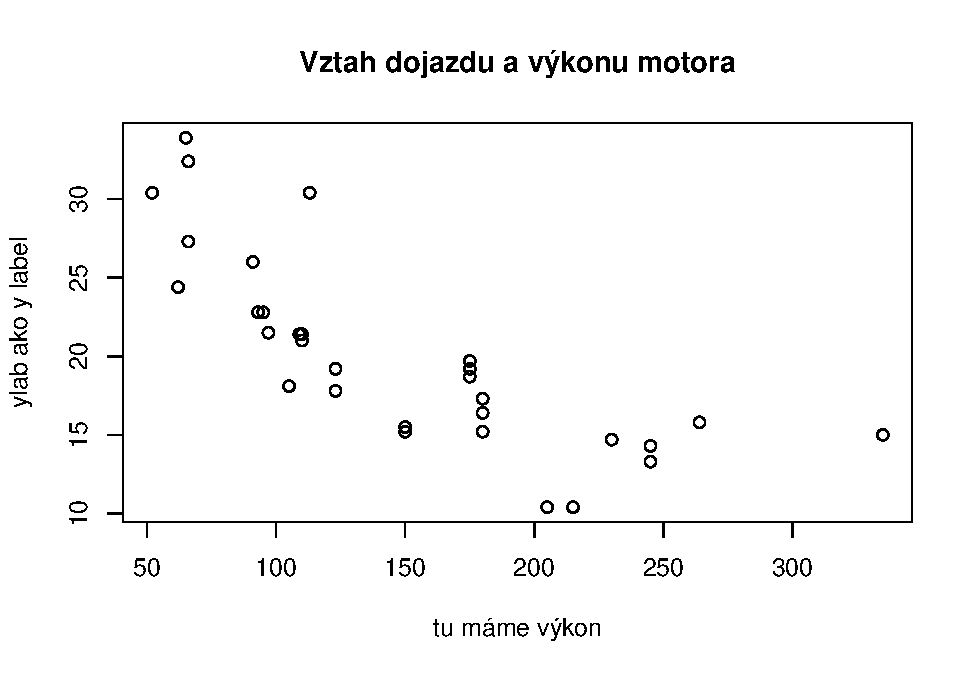
\includegraphics{test_files/figure-latex/unnamed-chunk-39-1.pdf}

Vidíme istú negatívnu závislosť. Chceli by sme si to však potvrdiť
číslami. Bolo by fajn napasovať medzi tieto pozorovania takú priamku,
ktorá bude ku každému pozorovaniu čo najbližšie. Keďže nepoznáme
parametre populácie, budeme pracovať s ich estimátormi, odhadcami.
Estimátory označíme striežkou ako \(\hat\beta_0{}\) a \(\hat\beta_1{}\).
Model bude vyzerať následovne:

\[\hat{mpg_i} = \hat\beta_0 + \hat \beta_1{hp_i}.\] Skúsme si takýto
model zostrojiť v R-ku, a priamku dopasovať do grafu.

\begin{Shaded}
\begin{Highlighting}[]
\CommentTok{# Chceme zistiť dopad "hp" na "mpg".}
\CommentTok{# Použijeme funkciu "lm()", ako linear model.}
\CommentTok{# Na konci musíme ako argument uviesť dáta, ktoré použijeme.}

\NormalTok{model <-}\StringTok{ }\KeywordTok{lm}\NormalTok{(mpg }\OperatorTok{~}\StringTok{ }\NormalTok{hp, }\DataTypeTok{data =}\NormalTok{ data)}

\CommentTok{# Alternatívne môžeme model napísať pomocou extrakcie takto.}
\CommentTok{# Preferujem tento postup.}

\NormalTok{model <-}\StringTok{ }\KeywordTok{lm}\NormalTok{(data}\OperatorTok{$}\NormalTok{mpg }\OperatorTok{~}\StringTok{ }\NormalTok{data}\OperatorTok{$}\NormalTok{hp)}

\CommentTok{# Dostaneme dva koeficienty. Jeden pre intercept Beta0 a druhý pre Beta1 ako "hp".}

\NormalTok{model}
\end{Highlighting}
\end{Shaded}

\begin{verbatim}
## 
## Call:
## lm(formula = data$mpg ~ data$hp)
## 
## Coefficients:
## (Intercept)      data$hp  
##    30.09886     -0.06823
\end{verbatim}

\begin{Shaded}
\begin{Highlighting}[]
\CommentTok{# Intercept sa väčšinou neinterpretuje, slúži len pre určenie počiatočnej hodnoty.}
\CommentTok{# Ak by sme koeficient interpretovali, mohli by sme povedať, že auto s nula koňmi}
\CommentTok{# prejde 30 míľ na galón. Koeficient B1 by sme interpretovali ako:}
\CommentTok{# "každá extra konská sila, zníži dojazd o -0.068 míle". }
\end{Highlighting}
\end{Shaded}

\begin{Shaded}
\begin{Highlighting}[]
\CommentTok{# Znova si plotneme dáta.}

\KeywordTok{plot}\NormalTok{(}\DataTypeTok{x =}\NormalTok{ data}\OperatorTok{$}\NormalTok{hp, }\DataTypeTok{y =}\NormalTok{ data}\OperatorTok{$}\NormalTok{mpg, }\DataTypeTok{ylab =} \StringTok{"Dojazd"}\NormalTok{, }\DataTypeTok{xlab =} \StringTok{"Výkon",}
\StringTok{     main = "}\NormalTok{Vzťah dojazdu a výkonu motora}\StringTok{")}

\StringTok{# A pomocou funkcie "}\KeywordTok{abline}\NormalTok{()}\StringTok{" napasujeme do grafu priamku modelu.}
\StringTok{# Abline ako priamka z bodu A do bodu B.}

\StringTok{abline(model) }
\end{Highlighting}
\end{Shaded}

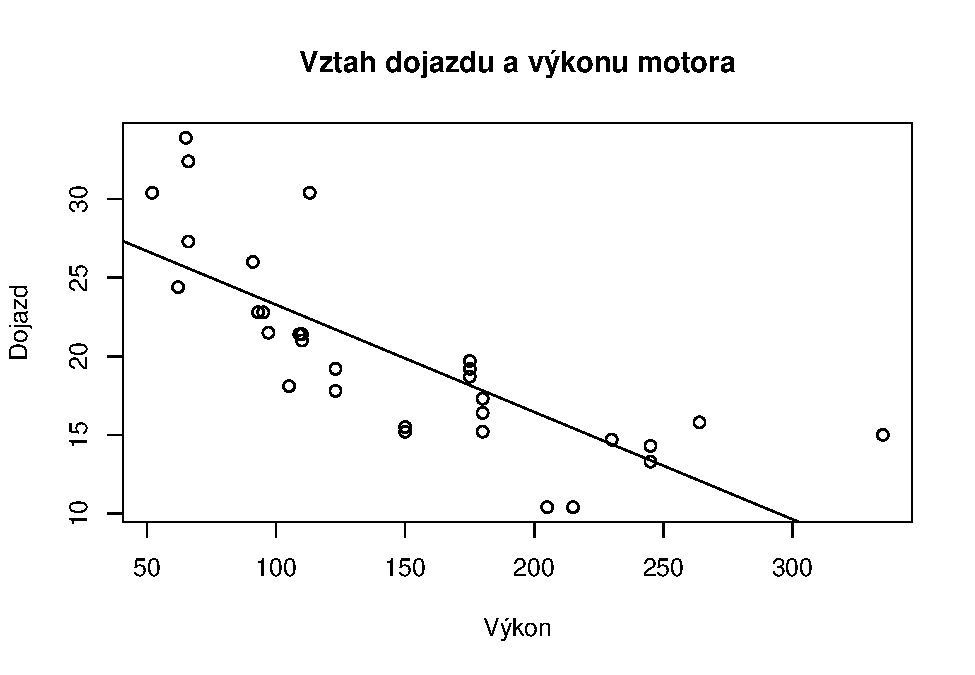
\includegraphics{test_files/figure-latex/unnamed-chunk-41-1.pdf}

Z grafu pozorujeme, že aj tu priamka neprechádza všetkými pozorovaniami,
túto kolmú vzdialenosť medzi priamkou a každým pozorovaním označíme ako
\(\hat{u}\). V tomto modeli to neoznačuje odhad náhodnej zložky
\(\epsilon\), ale výpočtovú nepresnosť modelu. Môžeme to brať ako takého
súrodenca k náhodnej zložke. Obe chyby predstavujú podobnú vec,
vzdialenosť medzi priamkou a pozorovaním. Priamku populácie je však
neznáma, teda aj táto vzdialenosť \(\epsilon\) je neznáma. Na druhú
stranu, zvyšky \(\hat{u}\) sú vyrátané z dát, a dokážeme ich presne
zmerať. Ako však vyrátame bety? Iste ste už začuli o OLS, teda Ordinary
Least Squares alebo Metódy najmenších štvorcov. Bety so striežkou
nazývame ako OLS estimátory. Metóda najmenších štvorcov sa to volá
preto, lebo vezmeme zvyšky \(\hat{u}\) z modelu, umocníme ich na druhú
mocninu (urobíme z nich štvorce), a minimalizujeme ich. Osobne si
nemyslím, že v tomto štádiu vašej výučby má veľký význam sústrediť sa na
odvodenie týchto estimátorov. Osobne mi to moc nedalo, preto sa skôr
zameriame na výsledky týchto odvodzovaní, nech nadobudneme trocha
intuície. Vysvetlíme si graficky, čo touto metódou chceme docieliť.

\begin{center}

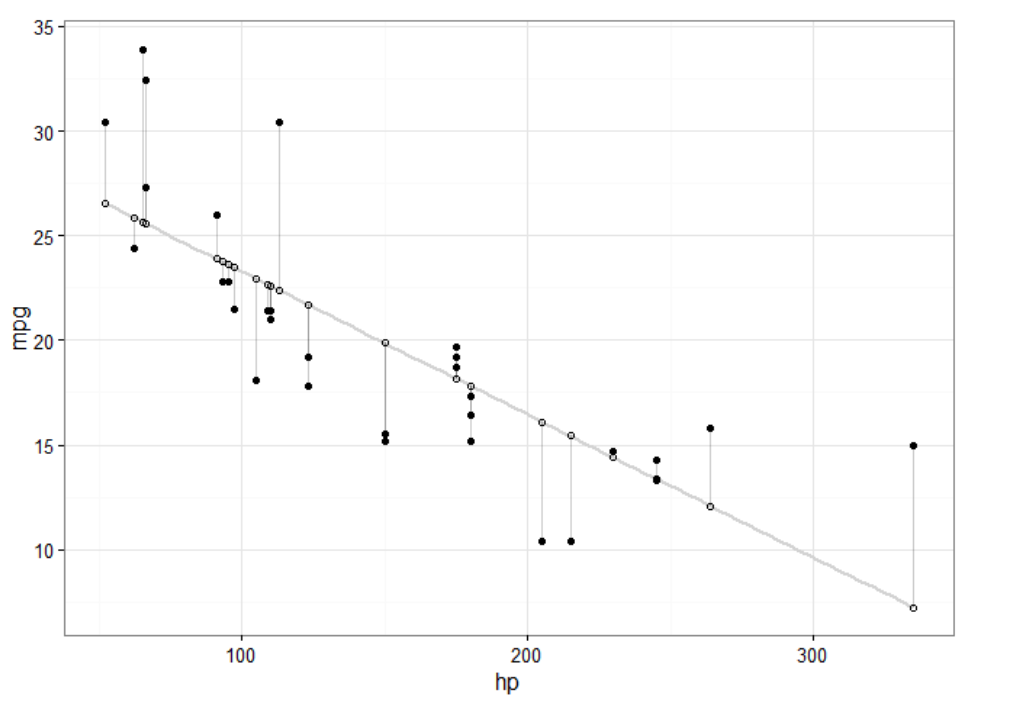
\includegraphics[width=0.85\textwidth,height=\textheight]{diplomka obrazky/4.png}

\end{center}

Tieto vzdialeností predstavujú naše ``residuals'' \(\hat{u}_i\), naše
zvyšky z modelu, naše nepresnosti. Každý data point má svoj zvyšok.
Logicky chceme, aby priamka čo najtesnejšie vystihovala dáta, chceme tým
pádom čo najviac zmenšiť zvyšky. Poďme sa k tým zvyškom dopracovať.

Pozorovanie sa rovná bodu na priamke \(\hat\beta_0 + \hat\beta{x}_i\)
plus zvyšok \(\hat{u}_i\):

\[ y_i = \hat\beta_0 + \hat\beta{x}_i + \hat{u}_i.\]

\begin{center}

Poprehadzujme si to, nech máme na jednej strane zvyšok \(\hat{u}_i\):

\end{center}

\[ \hat{u}_i = y_i - \hat\beta_0 - \hat\beta{x}_i.\]

Väčšinou narazíme na takýto zápis zvyškov, a to rozdiel medzi
pozorovanou hodnotou a odhadnutou hodnotou na priamke:

\[\hat{u}_i = y_i - \hat{y_i}.\]

\begin{center}

a keďže

\end{center}

\[ \hat{y}_i =\hat\beta_0 + \hat\beta{x}_i,\]

Tak sme tam, kde sme boli na začiatku, keď sme si dali zvyšok
\(\hat{u}_i\) na jednu stranu. OLS metódoa urobí to, že minimalizuje
súčet našich umocnených zvyškov \(\hat{u}_i\):

\[min\sum (y_i - \hat\beta_0 - \hat\beta_1{x}_i)^2.\]

Tým, že minimalizujeme zvyšky dostaneme čo najlepšiu priamku, ktorá bude
sedieť čo najtesnejšie s dátami. Táto minimalizácia nám poskytne vzorec
na výpočet OLS estimátorov. Estimátorov parametrov populácie. Bavíme sa
o odhadcoch priesečníka, \(\beta_0\), a sklonu, \(\beta_1\). A keď sa
bavíme o odhadcoch, píšeme ich ako \(\hat\beta_0\) a \(\hat\beta_1\).
Nech si pamätáte.

Na hodinách sa stretnete so vzorcom pre výpočet biet v maticovej forme.
A to:

\[Est(\beta) = \hat\beta = (X^TX)^{-1}X^Ty.\]

\begin{quote}
\emph{T-čka znamenajú transpose matice a -1 vyrátanie inverzie.}
\end{quote}

\begin{Shaded}
\begin{Highlighting}[]
\CommentTok{# Inverznu maticu vyrátame pomocou "solve()" a transpozíciu pomocou "t()".}
\CommentTok{# V R-ku by sme to vyrátali ako:}

\KeywordTok{solve}\NormalTok{(}\KeywordTok{t}\NormalTok{(X) }\OperatorTok\StringTok{ }\NormalTok{X) }\OperatorTok\StringTok{ }\KeywordTok{t}\NormalTok{(X) }\OperatorTok\StringTok{ }\NormalTok{y}\ErrorTok{)}
\end{Highlighting}
\end{Shaded}

Tento vzorec by som nazval funkčným, avšak určite nie intuitívnym.
Pracujete s ním preto, lebo:

\begin{itemize}
\tightlist
\item
  takáto forma je ľahšie spracovateľná pre výpočtovú techniku,
\item
  R-ko pri práci s datasetom ho aj tak pretvorí na maticu, predtým než
  podá výsledky,
\item
  tento vzorec funguje ako pre jednoduchú lineárnu regresiu (jedno Y a
  jedno X), tak aj pre viacnásobnú regresiu (jedno Y a viacero X).
\end{itemize}

Ono, R-ko to urobí všetko za Vás, samo vyráta všetky koeficienty, nuž
nechceli by ste vedieť, čo tá \(\hat\beta\) vlastne robí? Pri
jednoduchej lineárnej regresií dokážeme OLS beta estimátory zapísať aj
takto:

\[\hat\beta_0 = \overline{y} - (\hat\beta_1\overline{x})\]

\[\hat\beta_1 = \frac{\sum_{i=1}^{n} (x_i - \overline{x})(y_i - \overline{y})}{\sum_{i=1}^{n} (x_i - \overline{x})^2}\]

\begin{quote}
\emph{Čiara nad písmenom znamená priemer, teda ybar(takto to čítame) je
priemer všetkých hodnôt ``y'' v datasete.}
\end{quote}

Neopúšťajte ma. Ak Vám tento vzorec nie je povedomý, nič sa nedeje.
Pozrieme sa na to. Rozdeľme si to na vrch a spodok. Začneme menovateľom,
lebo je kratší, hm.

Súčet od i = 1 po n znamená, že vykonáme operáciu pre každé \(x\) v
datasete a výsledky operácií sčítame.

\begin{quote}
\emph{Summation znak sa nazýva grécky sigma.}
\end{quote}

Od každého \(x\) odčítame priemernú hodnotu \(\overline{x}\) a umocníme
to. Získame tým variabilitu okolo priemeru, inak povedané, ako veľmi sú
data v datasete rozptýlené. Dostaneme rozptyl. Je dôležité podotknúť, že
rozptyl kvôli umocneniu nikdy nebude záporný. Dôležité je to preto, lebo
vzťah v čitateli určuje, či je \(\beta\) pozitívna alebo negatívna.
Takže menovateľ neovplyvní kladnosť či zápornosť čitateľa.

Vzťah v čitateli vyzerá celkom podobne k tomu v menovateli, hm? A nie je
to náhoda. Vzťah v čitateli je obyčajná kovariancia, inak povedané,
spoločný rozptyl. Predstavuje závislosť medzi dvoma veličinami. Tento
vzťah neumocňujeme, pretože chceme vidieť, či bude závislosť pozitívna,
alebo negatívna.

\begin{quote}
\emph{Kovariancia či korelácia? Čo je čo? Korelácia je štandardizovaná
kovariancia. Obe vysvetľujú to isté, líšia sa len v rozsahu. Kovarianciu
predelíme násobkom smerodajných odchýlok x a y, a získame koreláciu.
Štandardizujeme to preto, aby sme sa vedeli orientovať, aký veľký je v
skutočnosti vzťah medzi premennými. Ak sa bavíme o kovariancii hmotnosti
v kilogramoch a dĺžky lietadla v metroch, výsledné hodnoty budú veľmi
vysoké. Ak budú kladné, budeme vedieť, že je medzi nimi lineárna
závislosť, ale nevieme aká veľká. Ak by sme porovnávali kovarianciu
kurzu EUR a USD, výsledné hodnoty budú síce menšie, ale stále o nič viac
vhodné na interpretovanie. Ak však tieto hodnoty predelíme násobkom
smerodajných odchýlok, teda ich štandardizujeme, výsledné hodnoty budú
porovnateľné pre akékoľvek premenné. Keďže ťažké a dlhé lietadlo bude
mať úmerne veľké smerodajné odchýlky, kdežto výmenný kurz bude mať
smerodajnú odchýlku prislúchajúcu hodnotám kurzu. Hodnoty v korelácií
budú spadať medzi hranice -1 a 1. Kde záporná hodnota predstavuje
negatívnu lineárnu závislosť, a naopak.}
\end{quote}

Pri odhade však nechceme hodnoty štandardizovať, ale vecne odhadnúť
použiteľné hodnoty koeficientov. \(\hat\beta_1\) si jednoducho zapíšeme
ako:

\[\hat\beta_1 = \frac{Cov(x, y)}{Var(x)}.\] Otestujme si, či to naozaj
funguje.

\begin{Shaded}
\begin{Highlighting}[]
\CommentTok{# Pripomeňme si hodnoty nášho modelu.}

\NormalTok{model}
\end{Highlighting}
\end{Shaded}

\begin{verbatim}
## 
## Call:
## lm(formula = data$mpg ~ data$hp)
## 
## Coefficients:
## (Intercept)      data$hp  
##    30.09886     -0.06823
\end{verbatim}

\begin{Shaded}
\begin{Highlighting}[]
\CommentTok{# Na poradí pri kovariancii nezáleží.}

\NormalTok{kovar <-}\StringTok{ }\KeywordTok{cov}\NormalTok{(data}\OperatorTok{$}\NormalTok{mpg, data}\OperatorTok{$}\NormalTok{hp)}

\NormalTok{rozptyl <-}\StringTok{ }\KeywordTok{var}\NormalTok{(data}\OperatorTok{$}\NormalTok{hp)}

\NormalTok{beta1 <-}\StringTok{ }\NormalTok{kovar}\OperatorTok{/}\NormalTok{rozptyl}

\KeywordTok{print}\NormalTok{(beta1)}
\end{Highlighting}
\end{Shaded}

\begin{verbatim}
## [1] -0.06822828
\end{verbatim}

\begin{Shaded}
\begin{Highlighting}[]
\CommentTok{# Oba parametre majú hodnotu -0.068 a rovnajú sa.}
\CommentTok{# Skúsme B0.}

\NormalTok{ybar <-}\StringTok{ }\KeywordTok{mean}\NormalTok{(data}\OperatorTok{$}\NormalTok{mpg)}
\NormalTok{xbar <-}\StringTok{ }\KeywordTok{mean}\NormalTok{(data}\OperatorTok{$}\NormalTok{hp)}

\NormalTok{beta0 <-}\StringTok{ }\NormalTok{ybar }\OperatorTok{-}\StringTok{ }\NormalTok{(beta1 }\OperatorTok{*}\StringTok{ }\NormalTok{xbar)}

\KeywordTok{print}\NormalTok{(beta0)}
\end{Highlighting}
\end{Shaded}

\begin{verbatim}
## [1] 30.09886
\end{verbatim}

\begin{Shaded}
\begin{Highlighting}[]
\CommentTok{# Sedí. :)}
\end{Highlighting}
\end{Shaded}

Oba parametre majú hodnotu -0.068 a rovnajú sa.

Nevravím, že sme objavili Ameriku, ale aspoň viete, že \(\hat\beta_0\)
je nejaký priemer \(y\) a od toho odčítame \(\hat\beta_1\) vynásobenú
priemerom \(x\). A neskrýva sa za tým žiaden ťažký imaginárny vzorec.
Taktiež, že \(\hat\beta_1\) je spoločný rozptyl závislej a nezávislej
premennej, vydelený rozptylom nezávislej premennej.

Ako však vieme, či estimátorom \(\hat\beta_0\) a \(\hat\beta_1\) môžeme
veriť?

\hypertarget{trocha-ux161tatistiky}{%
\section{Trocha štatistiky}\label{trocha-ux161tatistiky}}

Predtým, než si povieme o podmienkach lineárnej regresie Vás oboznámim s
pár záležitosťami, s ktorými sa stretnete, a napriek tomu, že sú pomerne
jednoduché by Vám zabrali dosť googlenia.

Prejdeme si:

\begin{itemize}
\tightlist
\item
  očakávanú hodnotu,
\item
  zákon veľkých čísel,
\item
  náhodný výber,
\item
  centrálna limitná veta,
\item
  normálne rozdelenie.
\end{itemize}

Možno ste si všimli, že pri interpretáciach koeficientov sa často
opakuje niečo v zmyysle:``V priemere nám pri zvýšeni bla bla bla
narastie o bla bla bla.'' To \textbf{v priemere} je veľmi podstatné.
Väčšinou pracujeme so vzorkami, ktoré boli zozbierané z populácie, ktorá
je pre nás neznáma. Ideálne boli vybrané náhodne, teda pozorovania vo
vzorke sú náhodnými veličinami, a štatistiky ktoré z nich vyrátame sú
potom tiež náhodné veličiny. Prečo je to podstatné sa dozvieme v
nasledujúcich konceptoch.

\begin{quote}
\_Keď sa bavíme o štatistikách, máme na mysli akúkoľvek hodnotu, ktorú
je možné vyrátať a opisuje niečo. Priemer je štatistika, rozptyl je
štatistika."
\end{quote}

\hypertarget{oux10dakuxe1vanuxe1-hodnota}{%
\subsection{Očakávaná hodnota}\label{oux10dakuxe1vanuxe1-hodnota}}

Spomínam si, ako som otvoril videa Bena Lamberta, a tam na mňa vyskočilo
hneď nejaké tlačené É-čko a rôzne kvačky. Veľké tlačené E znamená
expected value, teda očakávaná hodnota. Je to tak, ako to znie.
Očakávaná hodnota náhodnej premennej je jednoducho povedané priemer,
ktorý by sme vyrátali za dlhú dobu a pri niekoľkonásobnom opakovanom
výbere vzorky. Pre diskrétnu náhodnú premennú vyrátame túto hodnotu ako
vážený súčet, kde váha je určená pravdepodobnosťou výskytu. Vzorcom:

\[E(y)= y_1p_1 + y_2p_2 + ... + y_kp_k = \sum_{i=1}^{k}y_ip_i\]

A teraz príklad zo života na pochopenie. Prečo myslíte, sa hovorí
``Lucky Seven'', teda že sedmička je šťastné číslo? Je to preto, lebo
keď sčítate všetky kombinácie čísel na dvoch hracích kockách, najviac
hodnôt vyjde pre 7, teda aj pravdepodobnosť, že padne toto číslo je
väčšia, ako pri ostatných súčtoch. V priemere potom padne najviac ľudom
sedmička, ľudia si to všímajú a stavujú na sedmičky, alebo také niečo,
nie som moc na gambling.

\begin{center}

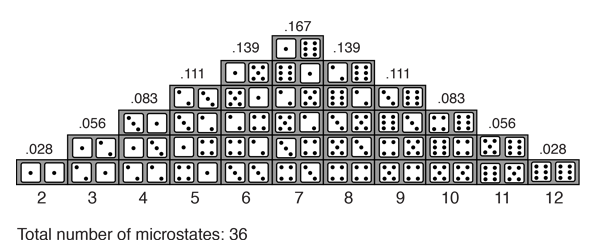
\includegraphics[width=0.8\textwidth,height=\textheight]{diplomka obrazky/5.png}

\end{center}

\hypertarget{zuxe1kon-veux13ekuxfdch-ux10duxedsel}{%
\subsection{Zákon veľkých
čísel}\label{zuxe1kon-veux13ekuxfdch-ux10duxedsel}}

S tým úzko súvisí aj zákon veľkých čísel. Zákon vraví, že ak rovnaký
experiment opakujeme nezávisle od seba nespočetne veľa krát, priemer
výsledkov bude blízko k \textbf{očakávanej hodnote}. Výsledok sa bude
približovať k očakávanej hodnote, ako sa bude počet pokusov zvyšovať.

\emph{Príklad:} Keď si s niekym budete hádzať mincu, možno padne 10-krát
za sebou orol, ale keby sme mincu hodili miliónkrát, výsledky by boli
približne 50/50. Inak povedané, šanca že padne hlava (alebo orol) je
50\%, ak minca nie je cinknutá. Očakávaná hodnota pri hode mincou je
0.5. Šanca že padne hlava je 1 a možné výsledky sú 2, teda
pravedpodobnosť, že padne hlava je 0.5, čiže 50\%.

\hypertarget{nuxe1hodnuxfd-vuxfdber-ux161tatistiky}{%
\subsection{Náhodný výber
štatistiky}\label{nuxe1hodnuxfd-vuxfdber-ux161tatistiky}}

V angličtine random sampling. To ing značí nejakú činnosť. Náhodný výber
znie skôr ako jeden výber, avšak pri random sampling ide o niečo iné.
Väčšina ekonometrických procedúr pracuje s priemermi vzoriek. Čiže tento
náhodný výber, sa bude týkať priemeru. Povedzme, že chceme odhadnúť
priemernú výšku v populácií. Väčšinou predpokladáme, že pozorovania sú
zozbierané náhodne z veľkej, nepoznanej populácie. Vyrátanie priemeru z
takejto vzorky má za následok to, že tento priemer je \emph{náhodnou
premennou}. \emph{Táto náhodná premenná má potom rozdelenie
pravdepodobnosti, nazývané výberové rozdelenie.} Výberové rozdelenie
závisí od rozdelenia populácie, z ktorej sme vzorku zobrali.
Predpokladajme, že máme normálne distribuovanú populáciu, a vyberieme z
nej veľa veľa vzoriek, vyrátame priemer týchto vzoriek, a urobíme z
týchto priemerov histogram. Rozdelenie tohto histogramu bude kopírovať
rozdelenie, z ktorého sme tieto vzorky zobrali, teda normálne
rozdelenie. Náhodný výber by mal eliminovať odchýlku, keďže každý z
populácie má rovnakú šancu byť vybraný. Získame teda rozdelenie bez
odchýlky, ktoré kopíruje rozdelenie populácie. Výberové rozdelenie môže
byť blízko normálneho rozdelenia, aj keď populácia z ktorej sme brali
vzorky nemá normálne rozdelenie. A to vďaka Centrálnej limitnej vete.

\hypertarget{centruxe1lna-limitnuxe1-veta}{%
\subsection{Centrálna limitná veta}\label{centruxe1lna-limitnuxe1-veta}}

Kdežto Zákon veľkých čísel sa zameriaval skôr na odhad danej štatistiky,
Centrálna limitná veta súvisí s rozdelením vzorky. Podstatou je, že ak
vezmeme dostatočne veľké množstvo priemerov vzoriek, súbor týchto
priemerov bude mať normálne rozdelenie, bez ohľadu na rozdelenie
populácie. Takáto vzorka by mala mať aspoň 30 pozorovaní. Nie je však
potrebné zbierať veľa veľa vzoriek, keďže na vzorku použijeme estimátor,
napríklad na odhad priemeru, a samotný výsledok bude náhodná veličina
(ako sme už spomenuli pri náhodnom výbere), ktorá sama pochádza z
náhodného výberu. Čiže na splnenie predpokladu, že výsledné rozdelenie
budeme môcť odhadnúť normálnym rozdelením, závisí už len od veľkosti
vzorky. Čím vzdialenejšie od normálneho rozdelenia je rozdelenie
populácie, tým väčšia vzorka bude potrebná, aby toto pravidlo platilo.

\hypertarget{podmienky-lineuxe1rnej-regresie}{%
\section{Podmienky lineárnej
regresie}\label{podmienky-lineuxe1rnej-regresie}}

My chceme, aby naše estimátory boli BLUE! A tým nemyslíme modré, ale
Best Linear Unbiased Estimators! Najlepší Lineárni Nevychýlení
Odhadcovia!

Unbiased znamena že v priemere Beta trafí cieľ, teda priemer.

\newpage

Vy sa učíte rátať toto pomocou solve x transpose, bude to fungovať aj na
SLR, avšak ukažeme si beta estimatory\ldots{} bla bla.. vyratame cov a
var.. rovno si naš model plotnime nech si ukažeme chyby. OLS sa snaži
napasovať priamku tak, aby boli chyby najmenšie. čiže residuals vs
fitted

\(\sideset{}{}\sum_{n=1}^{n}\)

\(\sum_{n=1}^{n}\)

\(\hat{\beta_0}\)

\[\hat{y} = a + bx\]

where

\[\hat{\beta_0} = \bar{y} - \hat{\beta_1} \bar{x}\] \#nainštalovat len
jeden balik a potom ked prejdeme vektory tak c(viac balikov)

\hypertarget{import-uxfadajov}{%
\subsection{Import údajov}\label{import-uxfadajov}}

Table Header

\begin{longtable}[]{@{}ll@{}}
\toprule
Fukncia & Second Header\tabularnewline
\midrule
\endhead
Content Cell & Content Cell\tabularnewline
Content Cell & Content Cell\tabularnewline
\bottomrule
\end{longtable}

\end{document}
